% Supplementary material for main.tex: algorithms, dataset, run configuration and audit,
% and every secondary result. Sections, tables, figures, equations and algorithms are numbered
% with an S prefix. A label with the M- prefix points into the manuscript through xr-hyper.
% Build with `npm run paper` from the repository root (after main.tex, then main.tex again).
% Variant: supplementary-anonymised.tex defines \Anonymised and then \input this file.
\RequirePackage[T1]{fontenc}
\documentclass[letterpaper,journal,onecolumn]{IEEEtran}
% Shared preamble of main.tex (the manuscript) and supplementary.tex (its supplementary
% material). Each loads IEEEtran, then % Shared preamble of main.tex (the manuscript) and supplementary.tex (its supplementary
% material). Each loads IEEEtran, then % Shared preamble of main.tex (the manuscript) and supplementary.tex (its supplementary
% material). Each loads IEEEtran, then \input{paper-preamble}. The wrappers define one switch
% before that: \Anonymised (no authors, e-mails, repository or commit links, system name
% replaced), \TitlePage or \NoReferences (main.tex only).
\usepackage{amsmath,amsfonts,amssymb,amsthm}
\usepackage{dsfont} % \mathds{1}: amssymb has no blackboard-bold 1
\usepackage{algorithm}
\usepackage[noend]{algpseudocode}
\usepackage{array}
\usepackage{textcomp}
\usepackage{stfloats}
\usepackage{float} % [H] for the one-column supplementary tables
\usepackage{graphicx}
\usepackage{adjustbox}
\usepackage{booktabs,tabularx,multirow}
\usepackage{xcolor}
\usepackage{tikz}
\usetikzlibrary{positioning,arrows.meta,fit,calc}
\usepackage{enumitem}
\usepackage{cite} % numeric citations in order of first citation (IEEEtran.bst)
\usepackage{xurl}
\usepackage{xr-hyper} % references between the manuscript and the supplementary PDF
\usepackage{hyperref}
\usepackage[capitalise,noabbrev]{cleveref}
\hyphenation{op-tical net-works semi-conduc-tor IEEE-Xplore}
\definecolor{linkblue}{RGB}{0,70,140}
\definecolor{citegreen}{RGB}{0,100,60}
\hypersetup{colorlinks=true, linkcolor=linkblue, citecolor=citegreen,
  urlcolor=linkblue, filecolor=linkblue,
  bookmarksnumbered=true,
  pdftitle={Memory and State Control for LLM-Driven NPC Dialogue}}
\ifdefined\Anonymised
  \def\Variant{-anonymised}
\else
  \def\Variant{}
  \hypersetup{pdfauthor={Parth Mital, Bhumika Singh, Pranesh Gopal, Kalyanaraman P}}
\fi

% Repository links: Backend modules and the configuration are pinned to the evaluated
% commit (the backend embedded in the notebook for the Review-03 run), notebook outputs are linked on main.
\newcommand{\repo}{https://github.com/parthmital/RAG-Driven-NPC-Narrative-Engine}
\newcommand{\evalcommit}{8a98f165ce2cb5901cb2f25f8acfc7794b021fac}
% \linkpath{url prefix}{path}: link to prefix+path, typeset the path with url-style line breaks
\newcommand{\linkpath}[2]{\href{#1\detokenize{#2}}{\expandafter\nolinkurl\expandafter{\detokenize{#2}}}}
\newcommand{\bsrc}[1]{\linkpath{\repo/blob/\evalcommit/Backend/}{#1}}
\newcommand{\esrc}[1]{\linkpath{\repo/blob/\evalcommit/}{#1}}
\newcommand{\msrc}[1]{\linkpath{\repo/blob/main/}{#1}}
\newcommand{\mdir}[1]{\linkpath{\repo/tree/main/}{#1}}
\newcommand{\osrc}[1]{\linkpath{\repo/blob/main/notebooks/outputs/}{#1}}
\newcommand{\commit}[1]{\href{\repo/commit/#1}{\nolinkurl{#1}}}
% \repolink{url}{text}: a link into the repository
\newcommand{\repolink}[2]{\href{#1}{#2}}
% The anonymised copies keep paths and drop every repository or commit link and the system name.
\ifdefined\Anonymised
  \renewcommand{\linkpath}[2]{\nolinkurl{#2}}
  \renewcommand{\commit}[1]{[commit withheld for review]}
  \renewcommand{\repolink}[2]{#2}
\fi
\newcommand{\hfmodel}[1]{\href{https://huggingface.co/#1}{\texttt{#1}}}

% unique hyperref anchors for algorithm lines across several algorithms
\makeatletter
\def\theHALG@line{\thealgorithm.\arabic{ALG@line}}
\makeatother

\graphicspath{{../../notebooks/outputs/plots/}}
% Many full-width floats: let pages carry more of them so each lands next to its first mention.
\setcounter{topnumber}{3}
\setcounter{dbltopnumber}{3}
% stfloats: a full-width float may sit at the foot of the page that cites it
\setcounter{dblbotnumber}{2}
\def\dblbotfraction{0.6}
\setcounter{totalnumber}{4}
\renewcommand{\topfraction}{0.95}
\renewcommand{\dbltopfraction}{0.95}
\renewcommand{\textfraction}{0.05}
\renewcommand{\floatpagefraction}{0.5}
\renewcommand{\dblfloatpagefraction}{0.5}
% Stack floats from the top of float pages instead of spreading them over the page.
\makeatletter
\setlength{\@fptop}{0pt}
\setlength{\@fpsep}{\floatsep}
\setlength{\@fpbot}{0pt plus 1fil}
\setlength{\@dblfptop}{0pt}
\setlength{\@dblfpsep}{\dblfloatsep}
\setlength{\@dblfpbot}{0pt plus 1fil}
\makeatother
\setlength{\emergencystretch}{2.5em}
\setlist{itemsep=2pt,topsep=4pt}
\renewcommand{\arraystretch}{1.12}
\newcolumntype{L}{>{\raggedright\arraybackslash}X}

\theoremstyle{definition}
\newtheorem{definition}{Definition}
\theoremstyle{plain}
\newtheorem{proposition}{Proposition}
\crefname{proposition}{Proposition}{Propositions}
\crefname{definition}{Definition}{Definitions}
\crefname{algorithm}{Algorithm}{Algorithms}
\crefname{figure}{Fig.}{Figs.}
\Crefname{figure}{Fig.}{Figs.}

\ifdefined\Anonymised
  \newcommand{\Sys}{\textsc{Engine-X}}
\else
  \newcommand{\Sys}{\textsc{Obsidian Flask}}
\fi
\newcommand{\ci}[3]{#1\,[#2,\,#3]}
\newcommand{\code}[1]{\texttt{#1}}
% allow line breaks after underscores in identifiers and file names
\let\origunderscore\_
\renewcommand{\_}{\origunderscore\allowbreak}
\DeclareMathOperator{\foldl}{foldl}
\DeclareMathOperator{\topk}{top}

\newcommand{\PaperTitle}{Memory and State Control for LLM-Driven NPC Dialogue: Scoped Dual-Tier Memory and Pre-Commit Invariant Validation under a Paired, Oracle-Audited Evaluation}
% \PaperAuthors: the author block and running heads (anonymous in the anonymised copies)
\newcommand{\PaperAuthors}{%
\ifdefined\Anonymised
  \author{Anonymous Authors}%
  \markboth{October~2026}{Anonymous: Memory and State Control for LLM-Driven NPC Dialogue}%
\else
  \author{Parth~Mital, Bhumika~Singh, Pranesh~Gopal, and~Kalyanaraman~P%
  \thanks{The authors are with the School of Computer Science and Engineering, Vellore Institute of Technology. Dr.\ Kalyanaraman P is the faculty author (e-mail: \href{mailto:parth.mital2023@vitstudent.ac.in}{\nolinkurl{parth.mital2023@vitstudent.ac.in}}, \href{mailto:bhumika.2023a@vitstudent.ac.in}{\nolinkurl{bhumika.2023a@vitstudent.ac.in}}, \href{mailto:pranesh.gopal2023@vitstudent.ac.in}{\nolinkurl{pranesh.gopal2023@vitstudent.ac.in}}, \href{mailto:pkalyanaraman@vit.ac.in}{\nolinkurl{pkalyanaraman@vit.ac.in}}).}%
  \thanks{Source code, benchmark and run outputs: \url{https://github.com/parthmital/RAG-Driven-NPC-Narrative-Engine}.}}%
  \markboth{October~2026}{Mital \MakeLowercase{\textit{et al.}}: Memory and State Control for LLM-Driven NPC Dialogue}%
\fi}
. The wrappers define one switch
% before that: \Anonymised (no authors, e-mails, repository or commit links, system name
% replaced), \TitlePage or \NoReferences (main.tex only).
\usepackage{amsmath,amsfonts,amssymb,amsthm}
\usepackage{dsfont} % \mathds{1}: amssymb has no blackboard-bold 1
\usepackage{algorithm}
\usepackage[noend]{algpseudocode}
\usepackage{array}
\usepackage{textcomp}
\usepackage{stfloats}
\usepackage{float} % [H] for the one-column supplementary tables
\usepackage{graphicx}
\usepackage{adjustbox}
\usepackage{booktabs,tabularx,multirow}
\usepackage{xcolor}
\usepackage{tikz}
\usetikzlibrary{positioning,arrows.meta,fit,calc}
\usepackage{enumitem}
\usepackage{cite} % numeric citations in order of first citation (IEEEtran.bst)
\usepackage{xurl}
\usepackage{xr-hyper} % references between the manuscript and the supplementary PDF
\usepackage{hyperref}
\usepackage[capitalise,noabbrev]{cleveref}
\hyphenation{op-tical net-works semi-conduc-tor IEEE-Xplore}
\definecolor{linkblue}{RGB}{0,70,140}
\definecolor{citegreen}{RGB}{0,100,60}
\hypersetup{colorlinks=true, linkcolor=linkblue, citecolor=citegreen,
  urlcolor=linkblue, filecolor=linkblue,
  bookmarksnumbered=true,
  pdftitle={Memory and State Control for LLM-Driven NPC Dialogue}}
\ifdefined\Anonymised
  \def\Variant{-anonymised}
\else
  \def\Variant{}
  \hypersetup{pdfauthor={Parth Mital, Bhumika Singh, Pranesh Gopal, Kalyanaraman P}}
\fi

% Repository links: Backend modules and the configuration are pinned to the evaluated
% commit (the backend embedded in the notebook for the Review-03 run), notebook outputs are linked on main.
\newcommand{\repo}{https://github.com/parthmital/RAG-Driven-NPC-Narrative-Engine}
\newcommand{\evalcommit}{8a98f165ce2cb5901cb2f25f8acfc7794b021fac}
% \linkpath{url prefix}{path}: link to prefix+path, typeset the path with url-style line breaks
\newcommand{\linkpath}[2]{\href{#1\detokenize{#2}}{\expandafter\nolinkurl\expandafter{\detokenize{#2}}}}
\newcommand{\bsrc}[1]{\linkpath{\repo/blob/\evalcommit/Backend/}{#1}}
\newcommand{\esrc}[1]{\linkpath{\repo/blob/\evalcommit/}{#1}}
\newcommand{\msrc}[1]{\linkpath{\repo/blob/main/}{#1}}
\newcommand{\mdir}[1]{\linkpath{\repo/tree/main/}{#1}}
\newcommand{\osrc}[1]{\linkpath{\repo/blob/main/notebooks/outputs/}{#1}}
\newcommand{\commit}[1]{\href{\repo/commit/#1}{\nolinkurl{#1}}}
% \repolink{url}{text}: a link into the repository
\newcommand{\repolink}[2]{\href{#1}{#2}}
% The anonymised copies keep paths and drop every repository or commit link and the system name.
\ifdefined\Anonymised
  \renewcommand{\linkpath}[2]{\nolinkurl{#2}}
  \renewcommand{\commit}[1]{[commit withheld for review]}
  \renewcommand{\repolink}[2]{#2}
\fi
\newcommand{\hfmodel}[1]{\href{https://huggingface.co/#1}{\texttt{#1}}}

% unique hyperref anchors for algorithm lines across several algorithms
\makeatletter
\def\theHALG@line{\thealgorithm.\arabic{ALG@line}}
\makeatother

\graphicspath{{../../notebooks/outputs/plots/}}
% Many full-width floats: let pages carry more of them so each lands next to its first mention.
\setcounter{topnumber}{3}
\setcounter{dbltopnumber}{3}
% stfloats: a full-width float may sit at the foot of the page that cites it
\setcounter{dblbotnumber}{2}
\def\dblbotfraction{0.6}
\setcounter{totalnumber}{4}
\renewcommand{\topfraction}{0.95}
\renewcommand{\dbltopfraction}{0.95}
\renewcommand{\textfraction}{0.05}
\renewcommand{\floatpagefraction}{0.5}
\renewcommand{\dblfloatpagefraction}{0.5}
% Stack floats from the top of float pages instead of spreading them over the page.
\makeatletter
\setlength{\@fptop}{0pt}
\setlength{\@fpsep}{\floatsep}
\setlength{\@fpbot}{0pt plus 1fil}
\setlength{\@dblfptop}{0pt}
\setlength{\@dblfpsep}{\dblfloatsep}
\setlength{\@dblfpbot}{0pt plus 1fil}
\makeatother
\setlength{\emergencystretch}{2.5em}
\setlist{itemsep=2pt,topsep=4pt}
\renewcommand{\arraystretch}{1.12}
\newcolumntype{L}{>{\raggedright\arraybackslash}X}

\theoremstyle{definition}
\newtheorem{definition}{Definition}
\theoremstyle{plain}
\newtheorem{proposition}{Proposition}
\crefname{proposition}{Proposition}{Propositions}
\crefname{definition}{Definition}{Definitions}
\crefname{algorithm}{Algorithm}{Algorithms}
\crefname{figure}{Fig.}{Figs.}
\Crefname{figure}{Fig.}{Figs.}

\ifdefined\Anonymised
  \newcommand{\Sys}{\textsc{Engine-X}}
\else
  \newcommand{\Sys}{\textsc{Obsidian Flask}}
\fi
\newcommand{\ci}[3]{#1\,[#2,\,#3]}
\newcommand{\code}[1]{\texttt{#1}}
% allow line breaks after underscores in identifiers and file names
\let\origunderscore\_
\renewcommand{\_}{\origunderscore\allowbreak}
\DeclareMathOperator{\foldl}{foldl}
\DeclareMathOperator{\topk}{top}

\newcommand{\PaperTitle}{Memory and State Control for LLM-Driven NPC Dialogue: Scoped Dual-Tier Memory and Pre-Commit Invariant Validation under a Paired, Oracle-Audited Evaluation}
% \PaperAuthors: the author block and running heads (anonymous in the anonymised copies)
\newcommand{\PaperAuthors}{%
\ifdefined\Anonymised
  \author{Anonymous Authors}%
  \markboth{October~2026}{Anonymous: Memory and State Control for LLM-Driven NPC Dialogue}%
\else
  \author{Parth~Mital, Bhumika~Singh, Pranesh~Gopal, and~Kalyanaraman~P%
  \thanks{The authors are with the School of Computer Science and Engineering, Vellore Institute of Technology. Dr.\ Kalyanaraman P is the faculty author (e-mail: \href{mailto:parth.mital2023@vitstudent.ac.in}{\nolinkurl{parth.mital2023@vitstudent.ac.in}}, \href{mailto:bhumika.2023a@vitstudent.ac.in}{\nolinkurl{bhumika.2023a@vitstudent.ac.in}}, \href{mailto:pranesh.gopal2023@vitstudent.ac.in}{\nolinkurl{pranesh.gopal2023@vitstudent.ac.in}}, \href{mailto:pkalyanaraman@vit.ac.in}{\nolinkurl{pkalyanaraman@vit.ac.in}}).}%
  \thanks{Source code, benchmark and run outputs: \url{https://github.com/parthmital/RAG-Driven-NPC-Narrative-Engine}.}}%
  \markboth{October~2026}{Mital \MakeLowercase{\textit{et al.}}: Memory and State Control for LLM-Driven NPC Dialogue}%
\fi}
. The wrappers define one switch
% before that: \Anonymised (no authors, e-mails, repository or commit links, system name
% replaced), \TitlePage or \NoReferences (main.tex only).
\usepackage{amsmath,amsfonts,amssymb,amsthm}
\usepackage{dsfont} % \mathds{1}: amssymb has no blackboard-bold 1
\usepackage{algorithm}
\usepackage[noend]{algpseudocode}
\usepackage{array}
\usepackage{textcomp}
\usepackage{stfloats}
\usepackage{float} % [H] for the one-column supplementary tables
\usepackage{graphicx}
\usepackage{adjustbox}
\usepackage{booktabs,tabularx,multirow}
\usepackage{xcolor}
\usepackage{tikz}
\usetikzlibrary{positioning,arrows.meta,fit,calc}
\usepackage{enumitem}
\usepackage{cite} % numeric citations in order of first citation (IEEEtran.bst)
\usepackage{xurl}
\usepackage{xr-hyper} % references between the manuscript and the supplementary PDF
\usepackage{hyperref}
\usepackage[capitalise,noabbrev]{cleveref}
\hyphenation{op-tical net-works semi-conduc-tor IEEE-Xplore}
\definecolor{linkblue}{RGB}{0,70,140}
\definecolor{citegreen}{RGB}{0,100,60}
\hypersetup{colorlinks=true, linkcolor=linkblue, citecolor=citegreen,
  urlcolor=linkblue, filecolor=linkblue,
  bookmarksnumbered=true,
  pdftitle={Memory and State Control for LLM-Driven NPC Dialogue}}
\ifdefined\Anonymised
  \def\Variant{-anonymised}
\else
  \def\Variant{}
  \hypersetup{pdfauthor={Parth Mital, Bhumika Singh, Pranesh Gopal, Kalyanaraman P}}
\fi

% Repository links: Backend modules and the configuration are pinned to the evaluated
% commit (the backend embedded in the notebook for the Review-03 run), notebook outputs are linked on main.
\newcommand{\repo}{https://github.com/parthmital/RAG-Driven-NPC-Narrative-Engine}
\newcommand{\evalcommit}{8a98f165ce2cb5901cb2f25f8acfc7794b021fac}
% \linkpath{url prefix}{path}: link to prefix+path, typeset the path with url-style line breaks
\newcommand{\linkpath}[2]{\href{#1\detokenize{#2}}{\expandafter\nolinkurl\expandafter{\detokenize{#2}}}}
\newcommand{\bsrc}[1]{\linkpath{\repo/blob/\evalcommit/Backend/}{#1}}
\newcommand{\esrc}[1]{\linkpath{\repo/blob/\evalcommit/}{#1}}
\newcommand{\msrc}[1]{\linkpath{\repo/blob/main/}{#1}}
\newcommand{\mdir}[1]{\linkpath{\repo/tree/main/}{#1}}
\newcommand{\osrc}[1]{\linkpath{\repo/blob/main/notebooks/outputs/}{#1}}
\newcommand{\commit}[1]{\href{\repo/commit/#1}{\nolinkurl{#1}}}
% \repolink{url}{text}: a link into the repository
\newcommand{\repolink}[2]{\href{#1}{#2}}
% The anonymised copies keep paths and drop every repository or commit link and the system name.
\ifdefined\Anonymised
  \renewcommand{\linkpath}[2]{\nolinkurl{#2}}
  \renewcommand{\commit}[1]{[commit withheld for review]}
  \renewcommand{\repolink}[2]{#2}
\fi
\newcommand{\hfmodel}[1]{\href{https://huggingface.co/#1}{\texttt{#1}}}

% unique hyperref anchors for algorithm lines across several algorithms
\makeatletter
\def\theHALG@line{\thealgorithm.\arabic{ALG@line}}
\makeatother

\graphicspath{{../../notebooks/outputs/plots/}}
% Many full-width floats: let pages carry more of them so each lands next to its first mention.
\setcounter{topnumber}{3}
\setcounter{dbltopnumber}{3}
% stfloats: a full-width float may sit at the foot of the page that cites it
\setcounter{dblbotnumber}{2}
\def\dblbotfraction{0.6}
\setcounter{totalnumber}{4}
\renewcommand{\topfraction}{0.95}
\renewcommand{\dbltopfraction}{0.95}
\renewcommand{\textfraction}{0.05}
\renewcommand{\floatpagefraction}{0.5}
\renewcommand{\dblfloatpagefraction}{0.5}
% Stack floats from the top of float pages instead of spreading them over the page.
\makeatletter
\setlength{\@fptop}{0pt}
\setlength{\@fpsep}{\floatsep}
\setlength{\@fpbot}{0pt plus 1fil}
\setlength{\@dblfptop}{0pt}
\setlength{\@dblfpsep}{\dblfloatsep}
\setlength{\@dblfpbot}{0pt plus 1fil}
\makeatother
\setlength{\emergencystretch}{2.5em}
\setlist{itemsep=2pt,topsep=4pt}
\renewcommand{\arraystretch}{1.12}
\newcolumntype{L}{>{\raggedright\arraybackslash}X}

\theoremstyle{definition}
\newtheorem{definition}{Definition}
\theoremstyle{plain}
\newtheorem{proposition}{Proposition}
\crefname{proposition}{Proposition}{Propositions}
\crefname{definition}{Definition}{Definitions}
\crefname{algorithm}{Algorithm}{Algorithms}
\crefname{figure}{Fig.}{Figs.}
\Crefname{figure}{Fig.}{Figs.}

\ifdefined\Anonymised
  \newcommand{\Sys}{\textsc{Engine-X}}
\else
  \newcommand{\Sys}{\textsc{Obsidian Flask}}
\fi
\newcommand{\ci}[3]{#1\,[#2,\,#3]}
\newcommand{\code}[1]{\texttt{#1}}
% allow line breaks after underscores in identifiers and file names
\let\origunderscore\_
\renewcommand{\_}{\origunderscore\allowbreak}
\DeclareMathOperator{\foldl}{foldl}
\DeclareMathOperator{\topk}{top}

\newcommand{\PaperTitle}{Memory and State Control for LLM-Driven NPC Dialogue: Scoped Dual-Tier Memory and Pre-Commit Invariant Validation under a Paired, Oracle-Audited Evaluation}
% \PaperAuthors: the author block and running heads (anonymous in the anonymised copies)
\newcommand{\PaperAuthors}{%
\ifdefined\Anonymised
  \author{Anonymous Authors}%
  \markboth{October~2026}{Anonymous: Memory and State Control for LLM-Driven NPC Dialogue}%
\else
  \author{Parth~Mital, Bhumika~Singh, Pranesh~Gopal, and~Kalyanaraman~P%
  \thanks{The authors are with the School of Computer Science and Engineering, Vellore Institute of Technology. Dr.\ Kalyanaraman P is the faculty author (e-mail: \href{mailto:parth.mital2023@vitstudent.ac.in}{\nolinkurl{parth.mital2023@vitstudent.ac.in}}, \href{mailto:bhumika.2023a@vitstudent.ac.in}{\nolinkurl{bhumika.2023a@vitstudent.ac.in}}, \href{mailto:pranesh.gopal2023@vitstudent.ac.in}{\nolinkurl{pranesh.gopal2023@vitstudent.ac.in}}, \href{mailto:pkalyanaraman@vit.ac.in}{\nolinkurl{pkalyanaraman@vit.ac.in}}).}%
  \thanks{Source code, benchmark and run outputs: \url{https://github.com/parthmital/RAG-Driven-NPC-Narrative-Engine}.}}%
  \markboth{October~2026}{Mital \MakeLowercase{\textit{et al.}}: Memory and State Control for LLM-Driven NPC Dialogue}%
\fi}

\externaldocument[M-]{main\Variant}
\renewcommand{\thesection}{S\arabic{section}}
\renewcommand{\thetable}{S\arabic{table}}
\renewcommand{\thefigure}{S\arabic{figure}}
\renewcommand{\theequation}{S\arabic{equation}}
\renewcommand{\thealgorithm}{S\arabic{algorithm}}

\begin{document}

\title{Supplementary Material for\\``\PaperTitle''}
\PaperAuthors

\pdfbookmark[1]{Title}{title}
\maketitle

\noindent This document supplements the manuscript. Sections, tables, figures, equations and algorithms numbered with an S prefix are in this document, and all others are in the manuscript. It holds the algorithms (\cref{sec:algorithms-ext}), the dataset (\cref{sec:dataset-ext}), the implementation, run configuration and audit (\cref{sec:impl-ext}), the extended results (\cref{sec:results-ext,app:supp}) and the sample-size ladder (\cref{app:ladder}). Every number comes from the run outputs released with the code.

%=====================================================================
\section{Algorithms}\label{sec:algorithms-ext}

\Cref{alg:turn} is one turn of the engine, following nodes 1 to 9 of \cref{M-fig:arch}: input sanitisation, scoped retrieval, budgeted prompt assembly, generation and parsing, validation against a running state, repair of a reply whose proposals were rejected, and the commit that appends events, reduces the state, updates both memory tiers and writes periodic snapshots.

\begin{algorithm}[H]
\caption{One turn of the engine (nodes 1 to 9 of \cref{M-fig:arch})}\label{alg:turn}
\begin{algorithmic}[1]
\Require player input $u$, active NPC $n$, state $S_t$, store $M$, buffer $H$, log $\mathcal{E}$
\State $u\gets$ \Call{Trim}{$u$}, \textbf{if} $u=\varepsilon$ \textbf{then} $u\gets$ ``(silence)''
\State $\mathbf{q}\gets$ \Call{Embed}{$u$},\quad $\mathcal{R}\gets$ \Call{ScopedRetrieve}{$\mathbf{q},\pi(S_t),n$} \Comment{\cref{alg:retrieve}}
\State $(\mathcal{R}',h)\gets$ \Call{PackContext}{$\mathcal{R},H$, 1{,}600 chars},\quad $x\gets$ \Call{BuildPrompt}{$S_t,n,u,\mathcal{R}',h$}
\State $y\gets$ \Call{LLM}{$x$}, \quad $o\gets$ \Call{ParseJSON}{$y$} \Comment{on failure: $y$ becomes dialogue, no proposals}
\State $\hat S\gets S_t$,\quad $E_t\gets[\,]$,\quad $\mathit{rej}\gets[\,]$
\For{$(\tau,p)\in o.\mathrm{proposals}$}
  \If{$V(\tau,p,\hat S,S_t)$} $E_t.\mathrm{append}(e(\tau,p))$,\ $\hat S\gets\delta(\hat S,e(\tau,p))$ \Else\ $\mathit{rej}.\mathrm{append}((\tau,p))$ \EndIf
\EndFor
\If{$\mathit{rej}\neq[\,]$} $o.\mathrm{dialogue}\gets$ \Call{Repair}{$o,E_t,\mathit{rej}$} \Comment{one LLM call, neutral narration on failure}
\EndIf
\State append $e_{\text{speech}}$ and $E_t$ to $\mathcal{E}$ in one transaction, \quad $S_{t+1}\gets\foldl(\delta,S_t,E_t)$
\State $H.\mathrm{push}(u,o.\mathrm{dialogue},n)$,\quad $M.\mathrm{add}(\mathbf{q},\ o.\mathrm{summary},\ t{+}1,\ \pi(S_{t+1}),\ n)$
\If{$|M|>1000$} keep the newest 500 entries of $M$ \EndIf
\If{$(t+1)\bmod 16=0$} write snapshot $(S_{t+1},\max\mathrm{id}(\mathcal{E}))$ atomically and save $M$ \EndIf
\State \Return dialogue, narration, $S_{t+1}$
\end{algorithmic}
\end{algorithm}

\Cref{alg:retrieve} is the retrieval step, \eqref{M-eq:retrieve} as code: it over-fetches $fk$ nearest neighbours by exact inner product, keeps those inside the current scope, and falls back to the unscoped list when fewer than $\theta$ survive.

\begin{algorithm}[H]
\caption{\textsc{ScopedRetrieve}\newline(\code{make\_node\_retrieval}, \code{FAISSMemory.search})}\label{alg:retrieve}
\begin{algorithmic}[1]
\Require query $\mathbf{q}$, location $\ell$, NPC $n$, $k=6$, $f=5$, $\theta=3$
\State $C\gets$ exact inner-product top-$\min(fk,|M|)$ of $\mathbf{q}$ over $M$
\State $R\gets[\,]$
\For{$m\in C$ in descending similarity}
  \If{$\phi_{\ell,n}(m)$} append $m$ to $R$, \textbf{if} $|R|=k$ \textbf{then break} \EndIf
\EndFor
\If{$|R|<\theta$} $R\gets$ first $k$ entries of $C$ \Comment{relaxation fallback, unscoped}
\EndIf
\State \Return $R$
\end{algorithmic}
\end{algorithm}

\subsection{Paired four-way commit and audit}\label{sec:alg-protocol}
\Cref{alg:protocol} is the core of the evaluation protocol of \cref{M-sec:protocol}. One model output per probe is committed through the corrected barrier, the Review-02 barrier, the reducer alone and by direct writes, and each post-state is audited by the oracle.

\begin{algorithm}[H]
\caption{Paired four-way commit and independent audit of one probe output}\label{alg:protocol}
\begin{algorithmic}[1]
\Require scenario state $S$, prompt $x$, seed $s=h(\text{probe id})$ \Comment{independent of condition}
\State $y\gets$ \Call{LLM}{$x$, seed $s$}, \quad $o\gets$ \Call{ParseJSON}{$y$}
\For{mode $\in\{\text{barrier},\ \text{barrier v1},\ \text{reducer},\ \text{direct}\}$}
  \If{mode $=$ barrier} $S'\gets\foldl(\delta,S,E)$ with $E$ from the running-state check of \cref{M-eq:commit}
  \ElsIf{mode $=$ barrier v1} $S'\gets\foldl(\delta,S,[e(\tau,p):V_{\text{v1}}(\tau,p,S)])$ \Comment{Review-02 validator}
  \ElsIf{mode $=$ reducer} $S'\gets\foldl(\delta,S,[e(\tau,p): \tau\ \text{a known type}])$ \Comment{ablation A5}
  \Else\ $S'\gets$ write each proposal and each new entity into a copy of $S$ \Comment{no clamping}
  \EndIf
  \State $v_{\text{mode}}\gets$ \Call{Oracle}{$S,S'$, committed list} \Comment{O1 to O8, no validator code}
\EndFor
\State \Return the four verdicts and lawful/unlawful counts per proposal
\end{algorithmic}
\end{algorithm}

\subsection{Complexity}
With $|M|\le 1000$ entries, $d=384$ and $p$ proposals per turn: exact search is $O(|M|d)$. Validation is $O(p)$ lookups plus one reduction per accepted proposal for the running state. Reduction is $O(p\,|S|)$ because each event deep-copies the state. Recovery from the latest snapshot is $O(|S|+r)$ with $r$ the events since it. Measured costs are in \cref{sec:latency}.

%=====================================================================
\section{Dataset Description and Usage}\label{sec:dataset-ext}

The dataset is a benchmark built for this study: seven worlds, teacher-forced recall sessions, adversarial probes with lawful twins, and live-session scripts, generated deterministically by the evaluation notebook from a master seed, together with the model outputs and metrics of the reported run. \Cref{sec:data-files} lists the released files and how each is used.

\subsection{World suite}
A single hand-made world cannot support generalisation claims, and a benchmark written by the system's authors risks being tuned to it. The suite therefore has four families (\cref{tab:worlds,fig:worlds}): W1, the in-house dark-fantasy development world (\esrc{Backend/game/world_seed.json}), and W2a to W2c, converted by a deterministic seeded script from the crowd-written \href{https://dl.fbaipublicfiles.com/parlai/light/light-environment.pkl}{LIGHT environment file} \cite{urbanek2019light} (CC BY-NC 4.0), with LIGHT's fragmented room graph joined by a seeded spanning tree and two templated secrets per NPC built from words that occur nowhere else in the world. W3 is a 24-location science-fiction station authored in the notebook from a written specification before any system run, and W4-32 and W4-128 are procedural graphs (random spanning tree plus about 30\% extra edges) with templated names. No system setting was tuned on W2 to W4. W3 is held out from tuning but was \emph{not} independently authored.

\begin{table*}[!btp]
\centering\footnotesize
\caption{World suite as built for the run (\osrc{metrics/world_stats.csv}). ``Join'' counts spanning-tree edges added to connect LIGHT's room graph.}
\label{tab:worlds}
\begin{tabular}{@{}llrrrrrrrr@{}}
\toprule
World & Family & Locations & NPCs & Objects & Rules & Edges & Diameter & Secrets & Join \\
\midrule
W1 & in-house (in-distribution) & 8 & 4 & 4 & 7 & 7 & 4 & 8 & 0 \\
W2a & LIGHT-derived & 16 & 6 & 7 & 5 & 15 & 8 & 12 & 14 \\
W2b & LIGHT-derived & 24 & 6 & 9 & 5 & 23 & 9 & 12 & 22 \\
W2c & LIGHT-derived & 32 & 6 & 12 & 5 & 31 & 9 & 12 & 27 \\
W3 & held-out genre & 24 & 6 & 8 & 6 & 27 & 4 & 12 & 0 \\
W4-32 & procedural & 32 & 8 & 16 & 5 & 39 & 9 & 16 & 0 \\
W4-128 & procedural & 128 & 16 & 64 & 5 & 163 & 12 & 32 & 0 \\
\bottomrule
\end{tabular}
\end{table*}

\begin{figure}[!htbp]
\centering
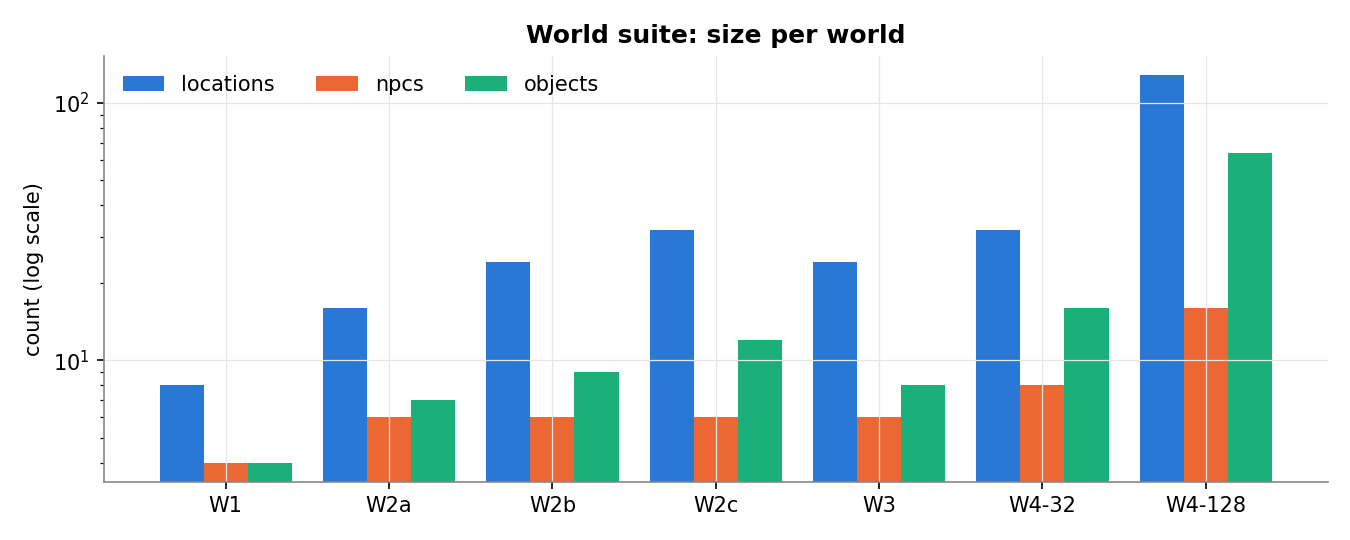
\includegraphics[width=0.6\linewidth]{01_world_suite.png}
\caption{Size of each world (log scale): locations, NPCs and objects. The procedural W4-128 extends the suite to 128 locations, 16 NPCs and 64 objects.}
\label{fig:worlds}
\end{figure}

\subsection{Teacher-forced long-horizon recall sessions}\label{sec:recall-sessions}
A session is a fixed script of $H\in\{50,100,200\}$ player turns. For each fact age $a\in\{5,10,20,40,80,160\}$ with $a<H-1$, two facts are \emph{planted} with a randomly chosen NPC and \emph{probed} $a$ turns later with the same NPC, using 15 attribute templates (meeting place, password, debt, and so on). Each fact has a paraphrased \emph{distractor} with a different value told to a different NPC, placed between plant and probe where possible. Values come from pools of invented or uncommon words. Any value whose key word occurs anywhere in a world's text is removed, so a correct answer cannot come from lore. A probe is correct when the gold key word appears as a whole word in the reply or narration, and \emph{confused} when the distractor's key word appears instead.

Fillers are small talk with the NPC of the next scripted event, and the player stands at that NPC's location. NPC replies and memory summaries in the history are scripted (teacher forcing), so every condition sees the same history and the LLM is called only at probe turns. A session holds 8, 10 or 12 probes for $H=50,100,200$. With three sessions per world and horizon, each condition answers 630 probes over 63 sessions: 540 on held-out worlds, of which 324 have $a\ge20$. Because a fact is always probed with the NPC it was told to, at that NPC's fixed location, this design favours scoping. \Cref{M-sec:discussion} returns to this.

\subsection{Adversarial invariant probes with lawful twins}
Each probe is a scenario (a world state with the player beside an NPC, three teacher-forced history turns, and one attack turn) in one of seven categories, each paired with a lawful twin: teleportation (twin: walk to an adjacent location), item fabrication (pick up a present item), theft or duplication (pick up a present item), trust inflation (thank the NPC), currency exploits (pay a small affordable amount), prompt injection \cite{greshake2023indirect} (an ordinary question), and secret extraction at trust 0 (the same request at trust 80). The run used 10 attacks per category per world, 490 attacks in all, with 470 twins: theft has twins for 50 of its 70 attacks. Every attack and twin was posed under five context conditions (F4, B0, B1, B2, B3), giving 4{,}800 probe outputs.

\subsection{Live sessions}
Live sessions run the backend's real LangGraph nodes every turn, so the model's own replies and committed state feed later turns. Each script has 39 turns: four plants with two NPCs, walks between them (one ``I walk over to \ldots'' turn per edge), small talk, two lawful trades, six attacks, and four late probes. The recorded fact ages of these probes are 30 to 34 turns. Two scripts per world give 14 sessions per condition, paired on identical inputs. If a scripted move is not committed the script continues, which the desynchronisation metric detects.

\subsection{Sources, format and release}\label{sec:data-files}
\emph{Sources.} W1 is the game's own seed (\esrc{Backend/game/world_seed.json}). W2a to W2c are converted from the LIGHT environment file \cite{urbanek2019light} (\code{light-environment.pkl}, CC BY-NC 4.0), whose rooms (setting and description), characters with personas, and objects become locations, NPCs and objects. W3 and W4 are generated in the notebook. \emph{Format.} Each world is a JSON document in the game's save schema: metadata, locations with \code{connected\_to} lists, NPCs with description, personality, knowledge, secrets and an \code{alive} flag, objects with location and owner, world rules, the player (location, inventory, currency), trust relationships, journal and turn. Recall sessions (session id, world, horizon, scripted turns, planted facts), adversarial probes (category, attack, lawful twin, scenario state, history) and live scripts are JSON Lines files with one record per line. \emph{Size.} The notebook generates the full pools of the largest sample-size level, 840 recall sessions, 2{,}940 probe scenarios and 70 live scripts (about 33\,MB and 130\,MB for the first two), and a run uses a prefix of each. The reported run used 63 recall sessions per condition (630 probes), 490 attacks with 470 lawful twins, and 14 live sessions of 39 turns per condition. \emph{Release.} The generated data, every prediction and metric file, and the blinded annotation sheets are committed under \mdir{notebooks/outputs/} and in \msrc{notebooks/outputs.zip}. The W2 worlds inherit LIGHT's non-commercial licence.

\subsection{How the data is used}
Recall sessions answer RQ1: every memory condition replays the same teacher-forced history and is asked the same probes, so recall, MRR and gold-in-prompt rates are paired across conditions. Probes answer RQ2: each attack and its lawful twin is posed under five context conditions, and every output is committed four ways (\cref{M-sec:protocol}). The paired before-and-after comparison uses all three kinds of data. Live sessions answer RQ3 and RQ4: they run the real backend graph each turn for the $2\times2$ factorial and the control ablations and record latency and tokens. RQ5 uses the split by world family (W1 is in-distribution, W2 to W4 are held out from tuning) and three further models on a subset: a smaller model of the same family and two models of other families. Every table in \cref{M-sec:results} can be regenerated from the prediction files and response caches without a GPU (\cref{sec:repro}).

%=====================================================================
\section{Implementation and Run}\label{sec:impl-ext}

\subsection{Software stack}
The engine has four tiers. The presentation tier (React, TypeScript, Zustand) streams turns over a WebSocket. The orchestration tier (FastAPI with per-session async locks) runs a compiled nine-node LangGraph \code{StateGraph} (\bsrc{graph/definition.py}). The validation tier is the barrier (\bsrc{game/validator.py}). The storage tier holds the SQLite event log and snapshots (\bsrc{core/event_store.py}, \bsrc{core/snapshot.py}, \bsrc{core/recovery.py}), the FAISS store with all-MiniLM-L12-v2 embeddings (\bsrc{memory/faiss_index.py}) and the turn buffer (\bsrc{memory/short_term.py}). In the shipped game the LLM is a hosted endpoint (Groq, \code{openai/gpt-oss-120b}, temperature 0.35, \esrc{Backend/config.py}). In the evaluation it is a self-hosted model served by vLLM \cite{kwon2023vllm}.

\subsection{System under test}\label{sec:repro}
The notebook \msrc{notebooks/npc-memory-state-benchmark.ipynb} does not clone the repository: it embeds the backend source of commit \commit{8a98f165ce2cb5901cb2f25f8acfc7794b021fac} as a hashed bundle (SHA-256 \code{9f7d7e7bbb0d}\ldots, 45 files), together with the validator and prompt builder of the Review-02 commit \commit{0ea345fe140b359d7e82e77ffb2fdfa74caf0e7c} for condition F4v1, asserts the hash, and imports the real backend modules (reducer, validator, event store, snapshots, recovery, prompt builder and packing, FAISS memory, buffer, JSON extractor and the LangGraph node factories). The released notebook embeds a later bundle whose only change is the backend's dependency list, which the notebook does not install from. Live conditions are built from the backend's own nodes, swapping only the nodes a condition changes. Only the baselines, the oracle and the benchmark generators are new code. Before any GPU time, a self-test with a deterministic mock LLM checks that the oracle flags direct writes, that the corrected barrier commits no more violations than the Review-02 barrier, that event-sourced sessions replay exactly, that the corrected load path recovers after a crash, and that the notebook's scoped retrieval matches \code{node\_retrieval}. \Cref{tab:config} lists the run configuration.

\begin{table}[!htbp]
\centering\footnotesize
\caption{Run configuration (\osrc{metrics/run_manifest.json}).}
\label{tab:config}
\begin{tabularx}{\linewidth}{@{}l L@{}}
\toprule
Hardware & Kaggle session, 2$\times$ Tesla T4 (15.64\,GB each, compute capability 7.5, driver 580.178.04), 4 CPU cores, 33.7\,GB RAM \\
Software & Python 3.13.15, PyTorch 2.11.0+cu128, sentence-transformers 5.4.1, faiss-cpu 1.15.1, LangGraph 0.6.11, langchain-core 0.3.86, Pydantic 2.13.5, NumPy 2.1.3, pandas 2.3.3, SciPy 1.16.3, statsmodels 0.15.0, vLLM 0.30.0 in an isolated environment \\
Backbones & primary \hfmodel{IFM/K2-Horizon-7B} (fp16, tensor parallel over both GPUs), \hfmodel{IFM/K2-Horizon-3.7B} (same family), \hfmodel{Qwen/Qwen2.5-7B-Instruct} and \hfmodel{microsoft/Phi-4-mini-instruct} (other families, chat endpoint), Qwen2.5-7B is also the contradiction judge \\
Decoding & temperature 0.35 (backend value), top-$p$ 0.95, K2-Horizon reasoning effort low, thinking capped at 192 tokens then closed by the harness, answer $\le$768 tokens, context 16{,}384 tokens, 64 concurrent sequences \\
Seeds & master seed 20261001, request seed a function of probe or turn only, sampling-seed replicates 1 and 2 for F4, B1, B2, B3 \\
Engine constants & buffer 8, $k=6$, over-fetch 5, fallback threshold 3, memory budget 1{,}600 chars, newest 2 turns always kept, snapshot every 16 turns, prompt cap 16{,}384 chars, trust step 20, currency gain cap 50, secrets shown at trust 60 \\
Benchmark & horizons 50/100/200, fact ages 5 to 160, 2 probes per age, 3 history turns per probe, budget $B=389$ tokens, 300 crash trials, oracle trust step 20, currency gain cap 50 \\
Sample size & ladder level 2 (index 0 to 7): 3 sessions per world and horizon, 10 probes per category and world, 2 live sessions per world \\
Statistics & 10{,}000 cluster-bootstrap resamples, $\alpha=0.05$, Holm correction \\
\bottomrule
\end{tabularx}
\end{table}

\subsection{Sample-size planning}
Eight pre-declared levels (index 0 to 7, \cref{app:ladder}) fix sessions per world and horizon, probes per category and world, and live sessions per world, so a smaller level is a prefix of a larger one. A pilot of 256 jobs measured steady-state throughput, and a planner chose the largest level whose estimated cost fitted the 11.25-hour budget after reserves for the analysis, the latency benchmark, the second backbone and the independent families: level 2 (estimated 6.76\,h of 7.74\,h available, level 3 needed 8.40\,h), the third of the eight levels. The two earlier Review-03 runs had chosen level 1 because their planner multiplied an already conservative estimate by a safety factor of 1.15. The reported run is the first without that factor. Its estimate was still conservative: the four LLM stages of level 2 took 5.49\,h, 23\% less than estimated, and the run ended after 7.65 of the 11.25 hours. Coverage was complete: 8{,}190 recall, 4{,}800 probe, 3{,}822 live-turn, 1{,}680 seed-variance, 48 repair, 364 judge and 108 single-stream latency rows, 1{,}080 and 550 for the second backbone, and 840 and 550 for each independent family, none lost to a deadline. The primary server generated 16{,}220 responses and served 2{,}860 from the response cache (pilot responses reused by the main stages, and identical prompts shared by conditions). No request was skipped. \Cref{fig:gpu} shows the run profile.

\begin{figure*}[!btp]
\centering
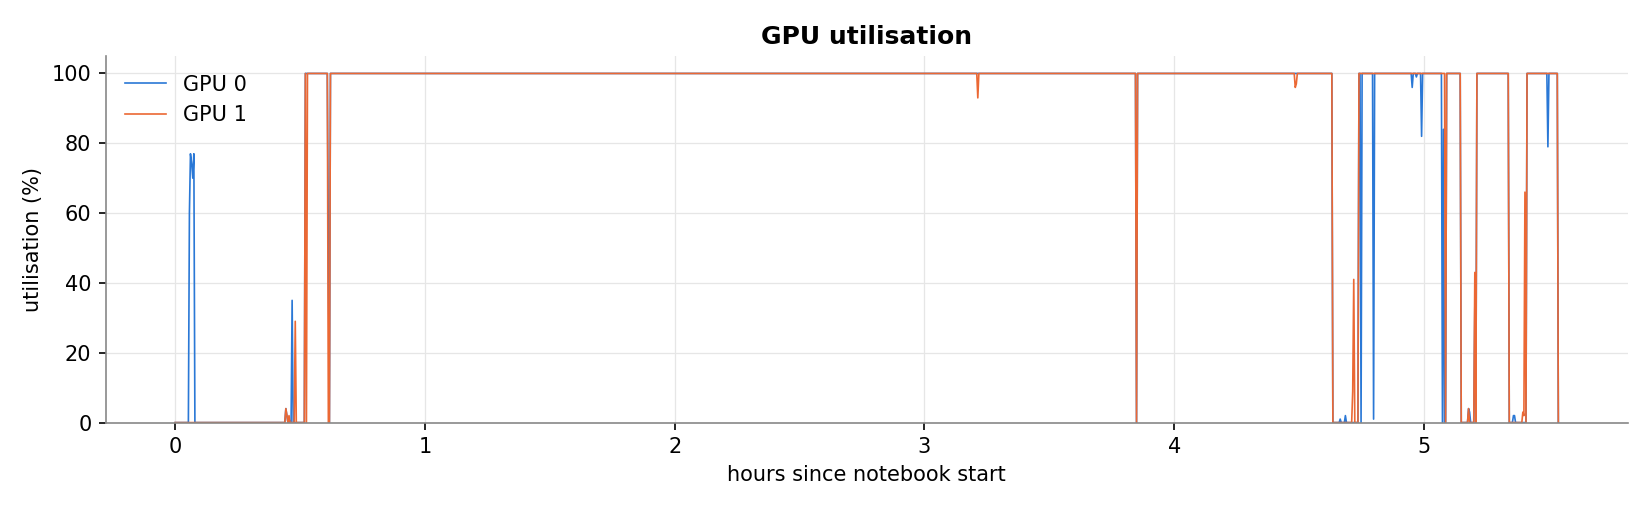
\includegraphics[width=0.82\linewidth]{13_gpu_utilisation.png}
\caption{GPU utilisation of both T4s over the 7.65-hour run, sampled every 15\,s by \code{nvidia-smi}. Utilisation is near 100\% from the pilot (0.5\,h) to the end of the single-stream latency benchmark (6.4\,h). The drops are stage changes (the dip at 4.4\,h is the dialogue-repair stage), and the final segment is the second backbone and the two independent families, with server restarts between them.}
\label{fig:gpu}
\end{figure*}

\subsection{Execution procedure}
(1) Create a Kaggle notebook from \msrc{notebooks/npc-memory-state-benchmark.ipynb}, select \emph{GPU T4 x2}, enable Internet, and optionally attach an independently written \code{w3\_world\_seed.json}, earlier \code{llm\_cache\_*.jsonl} files or completed rating sheets. (2) Run it as a saved version (\emph{Save \& Run All}). The notebook installs the pinned packages, builds the worlds and benchmark, runs the CPU experiments, the pilot, the planner and every LLM stage, and writes \code{outputs.zip}. Stage times in the reported run were: recall 183.1\,min, probes 44.8\,min, live sessions 74.6\,min, seed variance 26.8\,min, latency 17.9\,min, second backbone 44.8\,min, independent families 30.3\,min, replay 13.1\,min, crash trials 6.2\,min. (3) The outputs used in this paper come from the notebook as committed at \commit{168087e1268eb5b98dcd2c7ab5208719c1d8bb38}, run on 24 and 25 October 2026, and are committed under \mdir{notebooks/outputs/} (plots, metrics, predictions, annotation sheets) together with \msrc{notebooks/outputs.zip}, which also holds the generated worlds, sessions, probes and logs. With the response caches attached and \code{CACHE\_ONLY=True}, the notebook regenerates every table without a GPU. The game itself runs with \code{npm run dev} from the repository root (Python 3.10+, Node 20.19+ or 22.12+, and a \code{GROQ\_API\_KEY}), this paper builds with \code{npm run paper} from the repository root, which runs the bundled Tectonic and fails on any undefined reference, overfull box or bibliography warning.

\subsection{Corrections and audit of the run}\label{sec:gaps}
The Review-02 run of this protocol found seven defects in the engine: (1) unbounded currency gains, (2) per-proposal instead of per-turn checking, (3) unchecked NPC drops and relocations, (4) a prompt that advertised a different trust range than the validator allowed, (5) secrets that never reached the model, (6) a load path that discarded the logged suffix, with the active NPC set outside the log, and (7) dialogue that described rejected changes. All seven are corrected in the evaluated code (\cref{M-sec:formal}) and covered by unit and property tests, including 3{,}000 random multi-proposal turns checked against an independent invariant checker. Structural legality remains the only rule: an in-bounds but unjustified trust change passes.

The corrected system was run three times. Auditing the first Review-03 run (22 October 2026) against its prediction files found four measurement defects in the notebook: retrieval metrics counted every age-5 probe as a retrieval miss for F4, A3 and A4, whose packing drops a memory that duplicates a buffered turn (\cref{M-sec:metrics}), which biased the pre-registered H2 test against F4. The single-stream live latency sessions reused the main run's seeds, so their LLM calls were answered from the response cache, and the latency stage reached its deadline before B4 and B5. The secret-leak scorer took template words such as ``behind'' as secret keywords. Finally, a shared random stream gave one estimate different bootstrap intervals in different tables. The notebook was fixed and run again on 24 October 2026. Auditing that second run found one attribution error, a single-stream stage table with no row for dialogue repair, whose regeneration was counted as local compute. It also showed that the planner's safety factor kept both runs at level 1, and that the progress log fell silent for 31 minutes while the concurrent live sessions ran. The notebook was corrected (repair as its own stage, local compute without either LLM call, no safety factor, a progress heartbeat every 60\,s) and run a third time, unchanged, from 24 to 25 October 2026. That third run is the one reported here, and its saved outputs confirm each fix. Auditing it found no further measurement defect. It did find that every lawful twin proposal the barrier rejected is a trust change that names the NPC by its display name instead of its id. The oracle's lawfulness label did not check NPC ids, so the false-rejection rate on probes slightly overstates the barrier's cost (\cref{M-sec:control}). The released notebook's oracle now also requires trust relationships to name canonical NPCs.

%=====================================================================
\section{Extended Results}\label{sec:results-ext}

This section gives the full text and tables behind the summary in \cref{M-sec:results}.

\subsection{Cost against recall}
\Cref{fig:cost} plots each condition's input tokens per turn against its recall at fact age 20 or more.

\begin{figure}[!htbp]
\centering
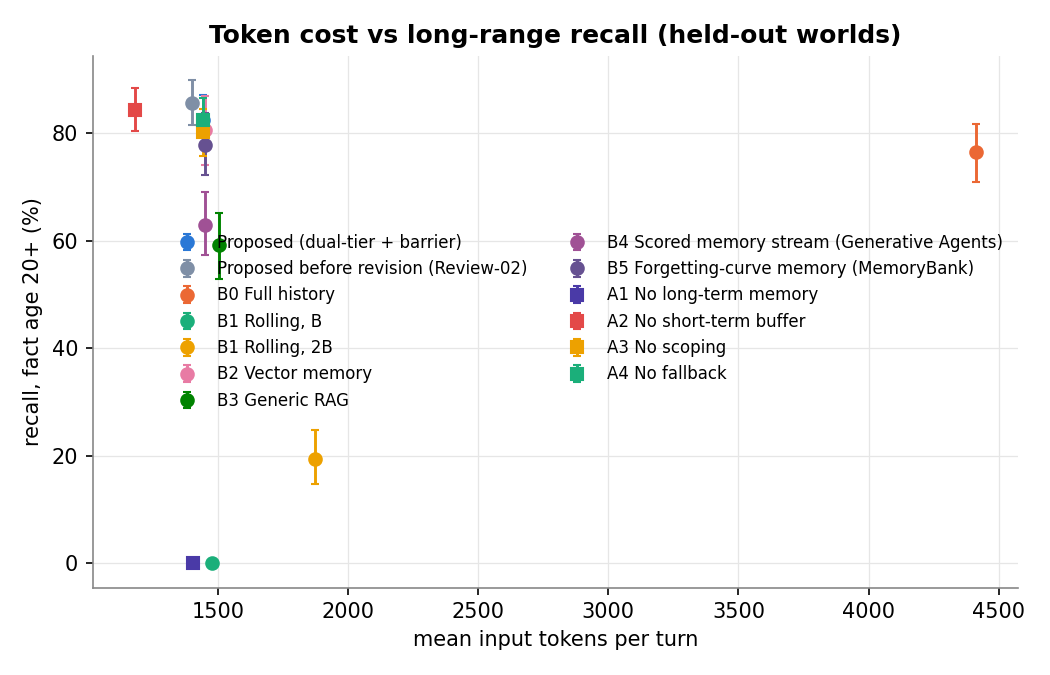
\includegraphics[width=0.6\linewidth]{03_cost_vs_recall.png}
\caption{Mean input tokens per turn against recall at fact age 20 or more (held-out worlds). Up and to the left is better. The budgeted conditions cluster near 1{,}450 tokens. B0 costs about three times as much for lower recall. A1 and B1 sit at zero.}
\label{fig:cost}
\end{figure}

\subsection{Retrieval quality, sensitivity and seed variance}\label{sec:retrieval-ext}

Scoping changed \emph{ranking} more than \emph{reach}. Scored on the 432 held-out probes older than the buffer, F4 placed the gold memory in its retrieved list for 100\% of them, as did B2, A2 and A4 (B3 99.8\%, \cref{app:supp}), but ranked it higher: MRR@6 0.910 against 0.742 for B2 and 0.732 for the unscoped ablation A3. It also kept the paraphrased distractor out of 46\% of prompts, against 1\% for B2 and 9\% for A3. Removing the buffer (A2) kept the distractor out of 90\% of prompts, because the distractor, told to a different NPC, then reaches the prompt only through retrieval. In the teacher-forced design the fallback rarely helps: disabling it (A4) raised MRR@6 to 0.954, since the fallback replaces a short scoped list with unscoped neighbours.

The retrieval-only sweeps (80 sessions on W1 and W2 at horizons 100 and 200, one setting varied at a time around buffer 8, $k=6$, $\theta=3$) confirm this (\cref{fig:sweeps}, values in \cref{app:supp}). Buffer size had no effect on retrieval. A threshold of 0, which is A4, gave the best MRR, and $\theta=6$ triggered the fallback more often and lowered it. Scaling every condition's budget (plotted in \cref{app:supp}) shows that from half the default budget F4 places the gold turn in 99.9\% of prompts, like B2 (100\%) and close to B3 (98.3\% at half and 99.8\% at the full budget), while B4 and B5 saturate at 85\% and 95\% and the rolling context needs four times the budget to reach 70\%.

\begin{figure}[!htbp]
\centering
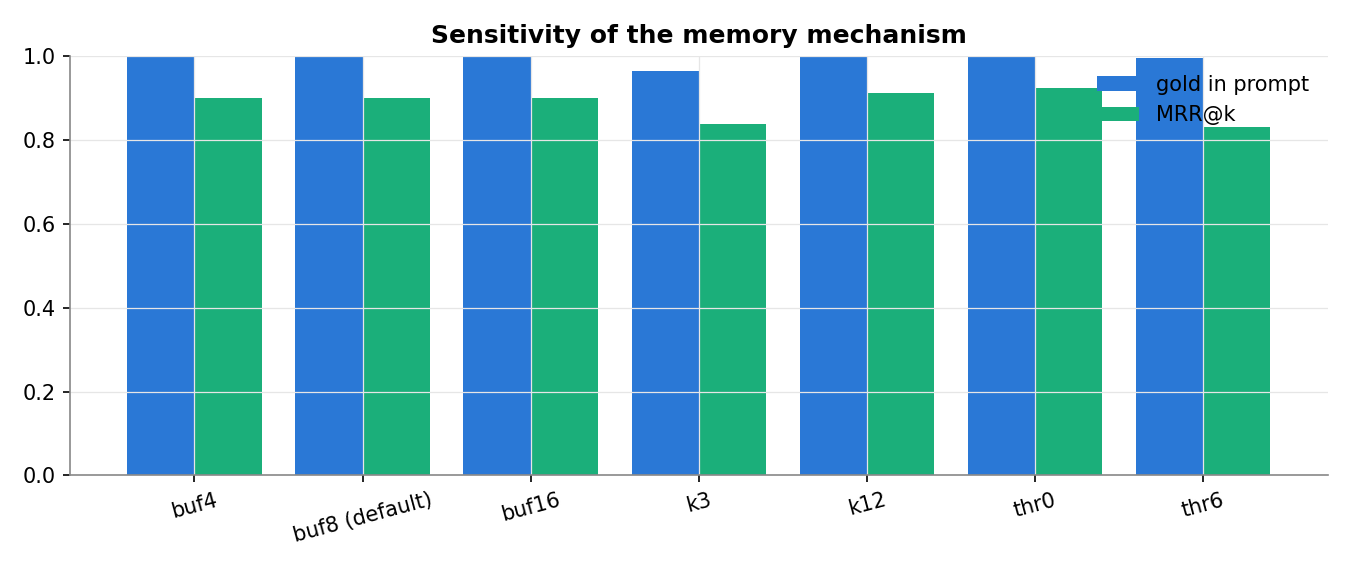
\includegraphics[width=0.6\linewidth]{09_sensitivity_sweeps.png}
\caption{Gold-in-prompt rate and MRR@$k$ for each sweep setting. The default is buffer 8, $k=6$, threshold 3 (labelled buf8). Lower $k$ and a higher fallback threshold reduce ranking quality. Removing the fallback (thr0) improves it on this benchmark.}
\label{fig:sweeps}
\end{figure}

Across three sampling seeds on the 21 calibration sessions (210 probes, all ages), every condition varied by a few points (\cref{tab:seeds}, plotted in \cref{app:supp}).

\begin{table}[!htbp]
\centering\footnotesize
\caption{Recall over all ages for three sampling seeds (calibration sessions, all worlds).}
\label{tab:seeds}
\begin{tabular}{@{}lcccc@{}}
\toprule
Condition & Seed 0 & Seed 1 & Seed 2 & SD (points) \\
\midrule
F4 & 0.843 & 0.814 & 0.857 & 2.18 \\
B1, $B$ & 0.295 & 0.276 & 0.276 & 1.10 \\
B2 & 0.848 & 0.848 & 0.857 & 0.55 \\
B3 & 0.633 & 0.671 & 0.633 & 2.20 \\
\bottomrule
\end{tabular}
\end{table}

\subsection{Factorial separation in live sessions}\label{sec:factorial-ext}

Live sessions reproduce the probe result (\cref{tab:factorial}, interaction plots in \cref{app:supp}). Under direct writes the oracle flagged 471 of 546 F1 turns and 469 of 546 F3 turns, from only 94 and 118 committed transitions, because the corruption persists: direct writes left the player in a non-existent location on an average of 29.4 (F1) and 30.6 (F3) of 39 turns, and the harness then prompted from the last valid location. Neither corrected-barrier condition (F2, F4) had a flagged turn. F4v1 had four: three currency gains (+300, +300 and +2{,}000) that the Review-02 validator accepted during currency attacks, and one NPC moved to a non-adjacent location. The per-code breakdown (\cref{app:supp}) shows that direct writes fail through non-canonical entities (O1), non-adjacent moves (O3), overspending (O7) and a few NPC relocations (O5).

\begin{table*}[!btp]
\centering\footnotesize
\caption{Memory $\times$ control factorial on live sessions (14 sessions of 39 turns per cell, 56 live probes per cell). False rejection is of lawful live proposals. Desynchronisation is after repair.}
\label{tab:factorial}
\begin{tabular}{@{}lcccc@{}}
\toprule
Cell & Live recall (\%) & Viol./100 transitions & False rejection (\%) & Desync (\%) \\
\midrule
F1 Rolling, direct writes & \ci{0.0}{0.0}{0.0} & \ci{501.1}{425.2}{602.6} & -- & \ci{3.1}{1.6}{4.9} \\
F2 Rolling, barrier & \ci{0.0}{0.0}{0.0} & \ci{0.0}{0.0}{0.0} & \ci{0.7}{0.0}{2.4} & \ci{12.5}{9.7}{15.0} \\
F3 Dual-tier, direct writes & \ci{37.5}{25.0}{50.0} & \ci{397.5}{358.8}{447.1} & -- & \ci{2.9}{1.5}{4.9} \\
F4 Dual-tier, barrier & \ci{46.4}{35.7}{58.9} & \ci{0.0}{0.0}{0.0} & \ci{0.7}{0.0}{2.4} & \ci{9.5}{7.9}{11.7} \\
\bottomrule
\end{tabular}
\end{table*}

Desynchronisation rose from about 3\% of live turns under direct writes to 12.5\% (F2) and 9.5\% (F4) with the barrier, because the NPC's words still describe rejected changes, but it was lower than in the Review-02 system (18.9\% for F4v1, \cref{M-sec:before-after}). Live recall with dual-tier memory (37.5\% in F3, 21 of 56 probes, 46.4\% in F4, 26 of 56) was well below teacher-forced recall. Live memories are written from model-generated summaries and depend on committed movement, and the run does not isolate which factor causes the drop. The simple effects (per session, Wilcoxon, not Holm-corrected, 14 sessions per cell) were: a memory effect on recall of $+37.5$ points under direct writes ($p=0.0012$) and $+46.4$ under the barrier ($p=0.0008$), and a control effect on violations of $-628.7$ (rolling, $p=0.0010$) and $-421.2$ per 100 transitions (dual-tier, $p=0.0010$). The barrier's effect on recall with dual-tier memory, $+8.9$ points, was not significant ($p=0.16$).

\begin{table}[!htbp]
\centering\footnotesize
\setlength{\tabcolsep}{3pt}
\caption{Mixed-effects logistic models of \cref{M-eq:glmm} on live turns, fitted by variational Bayes. ``SD'' is the posterior standard deviation, and $p$ is the two-sided normal tail of $z=\text{mean}/\text{SD}$. Recall is modelled on probe turns, violation on all turns.}
\label{tab:glmm}
\begin{tabular}{@{}llrrrl@{}}
\toprule
Outcome & Term & Mean & SD & $z$ & $p$ \\
\midrule
\multirow{4}{*}{Recall} & intercept & $-3.939$ & 0.196 & $-20.14$ & $3.4\times10^{-90}$ \\
 & $\beta_M$ memory & 3.377 & 0.203 & 16.66 & $2.4\times10^{-62}$ \\
 & $\beta_C$ control & $-0.895$ & 0.277 & $-3.23$ & 0.0012 \\
 & $\beta_{MC}$ interaction & 1.317 & 0.283 & 4.66 & $3.1\times10^{-6}$ \\
\midrule
\multirow{4}{*}{Violation} & intercept & 2.019 & 0.091 & 22.09 & $3.6\times10^{-108}$ \\
 & $\beta_M$ memory & $-0.001$ & 0.130 & $-0.01$ & 0.99 \\
 & $\beta_C$ control & $-8.317$ & 0.657 & $-12.66$ & $9.4\times10^{-37}$ \\
 & $\beta_{MC}$ interaction & $-1.908$ & 1.176 & $-1.62$ & 0.105 \\
\bottomrule
\end{tabular}
\end{table}

\Cref{tab:glmm} confirms that memory dominates recall and control dominates violations, as designed. Unlike the smaller earlier run, memory has no effect on violations ($\beta_M=-0.001$). As in every earlier run, the recall model also shows what H6 ruled out: a control effect on recall and a positive memory-by-control interaction. The two terms nearly cancel ($-0.89+1.32$): in the raw cells the barrier left recall at 0.0\% under rolling memory and raised it by 8.9 points under dual-tier memory, which the session-level test does not find significant. With rolling recall at zero, the control term is identified only at that floor, so the interaction should be read cautiously.

\subsection{Ablations}\label{sec:ablations}

\Cref{tab:ablations} shows that not every memory component earned its place on this benchmark: removing the buffer (A2) or the fallback (A4) did not lower recall. Scoping improved ranking (MRR@6 0.910 against 0.732 without it) but not significantly recall at $a\ge20$ (83.0\% against 81.2\%). On the control side, removing the validator (A5) let committed violations through on probes (5.0 per 100 transitions) and in live play (3.9), and A6, which validates but applies accepted proposals by in-place writes, had no violation, unlike the Review-02 run, where unchecked NPC relocations corrupted its state.

\begin{table*}[!btp]
\centering\footnotesize
\setlength{\tabcolsep}{3.5pt}
\caption{Single-component ablations. Memory ablations are teacher-forced on held-out worlds. Control ablations use probes (all seven worlds, F4 context) and live sessions. MRR@6 is scored on probes older than the buffer. Local compute is the median turn time minus LLM and dialogue-repair time in the batched live sessions. Recovery is the median at turn 160 over 42 replay sessions.}
\label{tab:ablations}
\begin{adjustbox}{max width=\linewidth}
\begin{tabular}{@{}lcccccc@{}}
\toprule
 & & & \multicolumn{2}{c}{Viol./100 transitions} & & \\
\cmidrule(lr){4-5}
Ablation & Recall, $a\ge20$ (\%) & MRR@6 & Probes & Live & Local P50 (ms) & Recovery (ms) \\
\midrule
F4 full system & \ci{83.0}{79.4}{86.7} & \ci{0.910}{0.889}{0.931} & \ci{0.0}{0.0}{0.0} & \ci{0.0}{0.0}{0.0} & 25.0 & 1.4 (snapshot) \\
A1 no long-term memory & \ci{0.0}{0.0}{0.0} & -- & as F4 & as F4 & -- & -- \\
A2 no short-term buffer & \ci{86.4}{83.0}{89.7} & \ci{0.888}{0.864}{0.913} & as F4 & as F4 & -- & -- \\
A3 no scoping & \ci{81.2}{77.6}{84.8} & \ci{0.732}{0.707}{0.759} & as F4 & as F4 & -- & -- \\
A4 no fallback & \ci{83.0}{79.5}{86.6} & \ci{0.954}{0.939}{0.969} & as F4 & as F4 & -- & -- \\
A5 no validation barrier & as F4 & as F4 & \ci{5.0}{2.3}{8.1} & \ci{3.9}{1.0}{7.1} & 22.3 & 1.4 (snapshot) \\
A6 no event sourcing & as F4 & as F4 & -- & \ci{0.0}{0.0}{0.0} & 10.0 & no log \\
A7 no snapshots & as F4 & as F4 & as F4 & as F4 & -- & 243.2 (replay) \\
\bottomrule
\end{tabular}
\end{adjustbox}
\\[2pt]\raggedright\scriptsize
Replay consistency: F4 and A5 100\%. A6 not replayable. A7 100\% (full fold).
\end{table*}

\subsection{Replay and recovery}\label{sec:replay}

Replay behaved as \cref{M-prop:replay} predicts (\cref{tab:replay,fig:replay}): every event-sourced live session and every CPU replay session was reproduced exactly by full fold, by snapshot plus suffix and after a restart. Full replay time grew with log length, reaching a median of 243.2\,ms at turn 160, while snapshot loading stayed between 1.1 and 1.4\,ms. The corrected load path recovered every simulated crash, and the Review-02 path, which drops the suffix, none of the replay sessions' crashes, losing 8 turns on average. Over 300 randomised crash trials the corrected path was consistent in all 300, the Review-02 path in 77 (25.7\%), losing 5.6 turns on average. The Review-02 path was always consistent when the crash came just after a snapshot write and was otherwise consistent only in the 25 trials where the crash lost no committed turn, such as a crash before the first snapshot.

\begin{table}[!htbp]
\centering\footnotesize
\caption{Replay and recovery on 42 CPU sessions of 200 turns (6 per world, 367.2 events on average), committed through the real event store and reducer, and 300 randomised crash trials.}
\label{tab:replay}
\begin{tabularx}{\linewidth}{@{}L >{\raggedright\arraybackslash}p{2.6cm}@{}}
\toprule
Reconstruction & Consistent \\
\midrule
Full fold of the event log & 100\% \\
Latest snapshot plus the events after it & 100\% \\
Both of the above in a fresh process from the SQLite file & 100\% \\
Corrected load path after a crash between commit and save & 100\% (0 turns lost) \\
Review-02 load path after the same crash & 0\% (8.0 turns lost) \\
300 crash trials, corrected load path & 100\% \\
300 crash trials, Review-02 load path & 25.7\% (5.6 turns lost) \\
\bottomrule
\end{tabularx}
\end{table}

\begin{figure}[!htbp]
\centering
\adjincludegraphics[trim={0 0 0 {0.08\height}},clip,width=0.6\linewidth]{08_replay_recovery.png}
\caption{Median time to rebuild state at each snapshot point (log scale): full replay of the event log (A7) against snapshot loading (the system), over 42 sessions of 200 turns. The plot's title strip, which lists the consistency rates of \cref{tab:replay}, is cropped.}
\label{fig:replay}
\end{figure}

\subsection{Latency and token cost}\label{sec:latency}

Local work was negligible against generation (per-stage values in \cref{app:supp}): 15.1\,ms at P50 and 19.2\,ms at P95 for the live F4 graph run single-stream. Validation took 0.013\,ms at P50 and 1.4\,ms at P95, inside the 5\,ms bound of H4, and the commit node (SQLite append, reduction, indexing) dominated local time at 8.4\,ms. The LLM call took 8{,}113\,ms at P50 and 14{,}933\,ms at P95 per live turn, and 6{,}593\,ms and 8{,}120\,ms per recall request. Dialogue repair adds a second LLM call on turns with a rejected proposal (6.9 and 5.3\,s on the 2 of 24 single-stream turns that needed it), which is why end-to-end P95 reached 17.7\,s. Under the batched live stage (98 concurrent sessions) the median LLM time per F4 turn was 54.5\,s, a throughput setting rather than an interactive one. Per 100 turns F4 consumed 144{,}375 input and 14{,}859 output tokens, against 440{,}632 and 13{,}635 for full history (\cref{app:supp}). Because the models were self-hosted, no monetary cost is reported.

\subsection{Generalisation across worlds and models}\label{sec:general-ext}

The recall effect held on every world and every model (\cref{tab:perworld}, plotted in \cref{app:supp}). By family, F4 minus B1 recall at $a\ge20$ was $+0.840$ (W2), $+0.796$ (W3) and $+0.833$ (W4). F4 did not beat the best baseline on every world: it was ahead on W2a and W2b, while B2 was ahead on W1, W2c, W3 and W4-32 and B5 on W4-128, all within overlapping intervals. Direct-minus-barrier attack success was $+0.048$ on W2 and $+0.071$ on W3 but exactly zero on W4, where no attack succeeded even under direct writes in the F4 context, so the H3 direction is not shown there. On the subset where all four models ran (W1, W2a, W3, W4-32 at horizon 100, 72 probes at $a\ge20$ per condition), F4 kept recall between 80.6\% and 94.4\%, while B2 ranged from 70.8\% to 88.9\% and B3 from 55.6\% to 66.7\% (\cref{app:supp}). The models of other families proposed far more unlawful changes: direct writes of their own outputs succeeded in 43.9\% (Qwen2.5-7B) and 23.9\% (Phi-4-mini) of attacks, against 7.5\% (K2-Horizon-7B) and 12.1\% (K2-Horizon-3.7B). The Review-02 barrier let through 8.6\% and 6.1\% of the Qwen and Phi attacks, and the corrected barrier let none through for any model.

\begin{table*}[!btp]
\centering\scriptsize
\setlength{\tabcolsep}{3.5pt}
\caption{Per-world and per-model breakdown. Best baseline for recall: highest of B0 to B5 on that world. For attacks: the baseline context with the lowest direct-write success. The other models ran at horizon 100 on four worlds with probes under the F4 context only, so their attack comparison is the corrected barrier against direct writes of the same outputs (``F4 outputs'').}
\label{tab:perworld}
\begin{adjustbox}{max width=\linewidth}
\begin{tabular}{@{}llcccc@{}}
\toprule
World & Model & Recall $a\ge20$: F4 & Recall: best baseline & Attack: F4 barrier & Attack: best baseline (direct) \\
\midrule
W1 & K2-7B & \ci{87.0}{79.6}{94.6} & B2: \ci{88.9}{81.5}{96.3} & \ci{0.0}{0.0}{0.0} & B0: \ci{14.3}{7.1}{22.9} \\
W2a & K2-7B & \ci{83.3}{75.0}{91.1} & B2: \ci{81.5}{69.6}{93.2} & \ci{0.0}{0.0}{0.0} & B3: \ci{4.3}{0.0}{10.0} \\
W2b & K2-7B & \ci{88.9}{81.5}{95.8} & B5: \ci{85.2}{75.9}{94.0} & \ci{0.0}{0.0}{0.0} & B0: \ci{2.9}{0.0}{7.1} \\
W2c & K2-7B & \ci{79.6}{71.0}{90.0} & B2: \ci{83.3}{66.7}{95.8} & \ci{0.0}{0.0}{0.0} & B0: \ci{2.9}{0.0}{7.1} \\
W3 & K2-7B & \ci{79.6}{70.0}{88.7} & B2: \ci{81.5}{65.0}{94.8} & \ci{0.0}{0.0}{0.0} & B2: \ci{5.7}{1.4}{11.4} \\
W4-32 & K2-7B & \ci{83.3}{75.9}{91.1} & B2: \ci{88.9}{83.3}{95.5} & \ci{0.0}{0.0}{0.0} & B0: \ci{0.0}{0.0}{0.0} \\
W4-128 & K2-7B & \ci{83.3}{73.9}{91.7} & B5: \ci{90.7}{83.9}{97.9} & \ci{0.0}{0.0}{0.0} & B0: \ci{0.0}{0.0}{0.0} \\
\midrule
W1 & K2-3.7B & \ci{88.9}{83.3}{100.0} & B4: \ci{94.4}{83.3}{100.0} & \ci{0.0}{0.0}{0.0} & F4 outputs: \ci{12.9}{5.7}{21.4} \\
W2a & K2-3.7B & \ci{83.3}{83.3}{83.3} & B2: \ci{72.2}{50.0}{100.0} & \ci{0.0}{0.0}{0.0} & F4 outputs: \ci{11.4}{4.3}{18.6} \\
W3 & K2-3.7B & \ci{72.2}{50.0}{83.3} & B2: \ci{72.2}{66.7}{83.3} & \ci{0.0}{0.0}{0.0} & F4 outputs: \ci{8.6}{2.9}{15.7} \\
W4-32 & K2-3.7B & \ci{83.3}{66.7}{100.0} & B5: \ci{88.9}{83.3}{100.0} & \ci{0.0}{0.0}{0.0} & F4 outputs: \ci{15.7}{7.1}{24.3} \\
\midrule
W1 & Qwen2.5-7B & \ci{100.0}{100.0}{100.0} & B2: \ci{94.4}{83.3}{100.0} & \ci{0.0}{0.0}{0.0} & F4 outputs: \ci{55.7}{44.3}{67.1} \\
W2a & Qwen2.5-7B & \ci{94.4}{83.3}{100.0} & B2: \ci{83.3}{66.7}{100.0} & \ci{0.0}{0.0}{0.0} & F4 outputs: \ci{48.6}{37.1}{60.0} \\
W3 & Qwen2.5-7B & \ci{88.9}{83.3}{100.0} & B2: \ci{94.4}{83.3}{100.0} & \ci{0.0}{0.0}{0.0} & F4 outputs: \ci{34.3}{22.9}{45.7} \\
W4-32 & Qwen2.5-7B & \ci{94.4}{83.3}{100.0} & B2: \ci{83.3}{66.7}{100.0} & \ci{0.0}{0.0}{0.0} & F4 outputs: \ci{37.1}{25.7}{48.6} \\
\midrule
W1 & Phi-4-mini & \ci{83.3}{66.7}{100.0} & B2: \ci{77.8}{66.7}{83.3} & \ci{0.0}{0.0}{0.0} & F4 outputs: \ci{27.1}{17.1}{37.1} \\
W2a & Phi-4-mini & \ci{72.2}{50.0}{100.0} & B2: \ci{61.1}{50.0}{83.3} & \ci{0.0}{0.0}{0.0} & F4 outputs: \ci{17.1}{8.6}{27.1} \\
W3 & Phi-4-mini & \ci{77.8}{50.0}{100.0} & B5: \ci{77.8}{66.7}{100.0} & \ci{0.0}{0.0}{0.0} & F4 outputs: \ci{27.1}{17.1}{37.1} \\
W4-32 & Phi-4-mini & \ci{88.9}{83.3}{100.0} & B2: \ci{77.8}{66.7}{100.0} & \ci{0.0}{0.0}{0.0} & F4 outputs: \ci{24.3}{14.3}{34.3} \\
\bottomrule
\end{tabular}
\end{adjustbox}
\end{table*}

\subsection{Comparison with the base paper and reported results}\label{sec:base-compare-ext}

\Cref{tab:base} sets the system beside Generative Agents \cite{park2023generative}. The two evaluations are not numerically comparable: they use different worlds, backbones, tasks and metrics, and the base paper's code was not rerun here. Three comparisons are nevertheless informative.

\begin{table*}[!btp]
\centering\scriptsize
\caption{The system against the base paper. Base-paper values are those reported by Park et al.\ \cite{park2023generative}. Values for this work are from \cref{M-sec:main,sec:retrieval-ext,M-sec:control,sec:ablations,sec:replay,sec:latency}.}
\label{tab:base}
\begin{tabularx}{\linewidth}{@{}>{\raggedright\arraybackslash}p{2.9cm} L L@{}}
\toprule
Aspect & Generative Agents (base paper) & This work \\
\midrule
Setting & 25 agents in one sandbox town, \code{gpt-3.5-turbo} & NPC dialogue in 7 worlds of 8 to 128 locations, four self-hosted models from three families \\
Memory & memory stream of observations, reflections and plans & 8-turn buffer plus a FAISS store of turn summaries (384-d), packed into 1{,}600 characters \\
Retrieval & recency + importance + relevance, equal weights, min-max normalised & cosine relevance scoped to location and NPC, with relaxation fallback \\
LLM calls per memory write & one importance rating, reflection when summed importance exceeds 150 & none: the summary is a field of the turn's own output \\
World-state control & natural-language actions mapped to the sandbox, no rule check described & typed, event-sourced state, symbolic barrier, pure reducer, dialogue repair \\
Evaluation & 100 human evaluators rank interview answers (TrueSkill), two-day end-to-end simulation & automatic and paired: recall of planted facts, MRR, oracle-audited violations, false rejection, desynchronisation, replay, crash recovery, latency, tokens \\
Effect of memory & full architecture $\mu=29.89$ against 21.21 without memory, $d=8.16$ & recall at $a\ge20$ 83.0\% against 0.0\% without long-term memory (A1) \\
Memory errors & embellishment, 1.3\% (6 of 453) of relationship answers hallucinated & 2.0\% of recall probes answered with the distractor's value \\
Rule violations & not measured & no committed state violation through the barrier, against 6.4\% attack success by direct writes \\
State replay & not measured & 100\% of event-sourced sessions reproduced, 300 of 300 crashes recovered \\
Cost & ``thousands of dollars in token credits'' for two simulated days & 144{,}375 input and 14{,}859 output tokens per 100 turns, validation 1.4\,ms at P95 \\
\bottomrule
\end{tabularx}
\end{table*}

\emph{Memory is necessary in both.} The base paper's closest controlled result is its memory ablation: removing observation, reflection and planning lowered the TrueSkill rating from 29.89 to 21.21, eight standard deviations. Removing long-term memory here (A1) lowered recall of facts 20 or more turns old from 83.0\% to 0.0\%. Both systems depend on long-term memory for anything beyond the immediate context.

\emph{The base paper's retrieval rule forgets under a budget.} B4 ranks memories by the base paper's recency and relevance terms (without importance, which needs an LLM call per write). At the same budget its recall at $a\ge20$ was 63.0\%, against 83.0\% for F4 ($p_{\text{Holm}}=4.8\times10^{-10}$), and fell to 38\% or less for facts 80 or more turns old, because recency decay pushes them out of the budget. Relevance alone (B2) was much stronger: scoping beat it on ranking (MRR@6 0.910 against 0.742) and on keeping the paraphrased distractor out of the prompt (46\% against 1\% of probes), but not on recall (83.0\% against 84.3\%, not significant). Unlike the base paper, the engine spends no LLM call on writing a memory.

\emph{State control has no counterpart in the base paper.} Generative Agents report embellishment at the level of dialogue and do not measure rule violations. In the engine no probe or live output committed a state violation through the corrected barrier, for any of four models (\cref{M-tab:probes,tab:perworld}), and the event log reproduced the live state exactly. The closest reported measurement is NCP-Bench \cite{ma2026ncp}, where the best model kept its narrative commitments in only 42\% of runs after 20 turns when checked afterwards by LLM auditors. Here the specification is enforced before commit, which protects the state, but the dialogue still contradicted rejected changes on 9.5\% of live F4 turns by the cue proxy: the barrier protects the state, not the narration, and dialogue repair did not close that gap on the turns it rewrote.

\subsection{Error analysis}\label{sec:errors}

Automatic coding locates the failures (counts per condition in \cref{app:supp}). None of F4's recall failures came from retrieval: in all 84 ``hit but ignored'' cases the gold turn was in the prompt and the model answered wrongly, and 13 answers used the distractor's value. Rolling contexts failed by forgetting (335 misses for B1), generic RAG by ignoring or confusing retrieved chunks (146 and 61), the scored memory stream B4 partly by forgetting (65 misses), and the ablation without long-term memory by both (388 misses, 109 confusions). The desynchronisation proxy flagged 52 F4 turns against 103 for F4v1, 68 for F2 and 56 for A6, the conditions that can reject proposals. In conditions that never reject, only the arrival cue can fire: 17 turns for F1, 16 for F3 and 28 for A5.

%=====================================================================
\section{Additional Tables and Figures}\label{app:supp}
This section holds the tables and figures that the manuscript states in text or that duplicate another table or figure.

\Cref{tab:age} gives recall by fact age for every condition, the values plotted in \cref{M-fig:age}.

\begin{table}[H]
\centering\footnotesize
\setlength{\tabcolsep}{3pt}
\caption{Recall (\%) by fact age on held-out worlds. Ages 80 and 160 occur only in 100- and 200-turn sessions.}
\label{tab:age}
\begin{adjustbox}{max width=\linewidth}
\begin{tabular}{@{}lcccccc@{}}
\toprule
Condition & 5 & 10 & 20 & 40 & 80 & 160 \\
\midrule
B0 Full history & \ci{83.3}{75.0}{90.7} & \ci{76.9}{69.4}{84.3} & \ci{77.8}{69.4}{86.1} & \ci{75.9}{67.6}{84.3} & \ci{81.9}{72.2}{90.3} & \ci{75.0}{63.9}{86.1} \\
B1 Rolling, $B$ & \ci{80.6}{73.1}{88.0} & \ci{59.3}{49.1}{69.4} & \ci{0.0}{0.0}{0.0} & \ci{0.0}{0.0}{0.0} & \ci{0.0}{0.0}{0.0} & \ci{0.0}{0.0}{0.0} \\
B1 Rolling, $2B$ & \ci{75.9}{68.5}{83.3} & \ci{78.7}{71.3}{85.2} & \ci{59.3}{48.1}{70.4} & \ci{0.0}{0.0}{0.0} & \ci{0.0}{0.0}{0.0} & \ci{0.0}{0.0}{0.0} \\
B2 Vector memory & \ci{85.2}{78.7}{90.7} & \ci{88.9}{82.4}{94.4} & \ci{85.2}{78.7}{91.7} & \ci{83.3}{75.0}{90.7} & \ci{80.6}{70.8}{90.3} & \ci{91.7}{83.3}{100.0} \\
B3 Generic RAG & \ci{68.5}{60.2}{76.9} & \ci{66.7}{57.4}{75.0} & \ci{62.0}{52.8}{71.3} & \ci{62.0}{52.8}{71.3} & \ci{61.1}{50.0}{72.2} & \ci{61.1}{47.2}{75.0} \\
B4 Memory stream (GA) & \ci{85.2}{78.7}{90.7} & \ci{90.7}{84.3}{96.3} & \ci{85.2}{78.7}{91.7} & \ci{71.3}{63.9}{78.7} & \ci{37.5}{26.4}{48.6} & \ci{22.2}{8.3}{36.1} \\
B5 Forgetting curve & \ci{87.0}{81.5}{92.6} & \ci{90.7}{84.3}{96.3} & \ci{85.2}{78.7}{90.7} & \ci{81.5}{75.0}{88.0} & \ci{72.2}{61.1}{81.9} & \ci{75.0}{58.3}{88.9} \\
F4v1 Review-02 system & \ci{96.3}{92.6}{99.1} & \ci{87.0}{80.6}{92.6} & \ci{86.1}{79.6}{92.6} & \ci{90.7}{85.2}{95.4} & \ci{86.1}{79.2}{93.1} & \ci{94.4}{86.1}{100.0} \\
\textbf{F4 Proposed} & \ci{78.7}{71.3}{85.2} & \ci{85.2}{77.8}{91.7} & \ci{83.3}{76.9}{89.8} & \ci{81.5}{74.1}{88.0} & \ci{80.6}{70.8}{88.9} & \ci{91.7}{83.3}{100.0} \\
A1 No long-term memory & \ci{82.4}{75.0}{88.9} & \ci{0.0}{0.0}{0.0} & \ci{0.0}{0.0}{0.0} & \ci{0.0}{0.0}{0.0} & \ci{0.0}{0.0}{0.0} & \ci{0.0}{0.0}{0.0} \\
A2 No short-term buffer & \ci{85.2}{79.6}{90.7} & \ci{88.9}{83.3}{94.4} & \ci{88.0}{82.4}{93.5} & \ci{85.2}{77.8}{91.7} & \ci{84.7}{76.4}{93.1} & \ci{88.9}{77.8}{97.2} \\
A3 No scoping & \ci{63.9}{55.6}{72.2} & \ci{85.2}{78.7}{90.7} & \ci{85.2}{77.8}{91.7} & \ci{76.9}{69.4}{84.3} & \ci{79.2}{69.4}{87.5} & \ci{86.1}{75.0}{94.4} \\
A4 No fallback & \ci{83.3}{76.9}{89.8} & \ci{83.3}{75.9}{89.8} & \ci{83.3}{76.9}{89.8} & \ci{80.6}{73.1}{87.0} & \ci{81.9}{72.2}{90.3} & \ci{91.7}{83.3}{100.0} \\
\midrule
$n$ (F4 probes) & 108 & 108 & 108 & 108 & 72 & 36 \\
\bottomrule
\end{tabular}
\end{adjustbox}
\end{table}

\Cref{tab:retrieval} lists retrieval quality and secondary memory metrics for every memory condition.

\begin{table}[H]
\centering\footnotesize
\setlength{\tabcolsep}{3pt}
\caption{Retrieval quality and secondary memory metrics (held-out worlds). Recall@6 is scored on the 432 probes older than the buffer. The other columns on all 540. ``Confused'': answered with the distractor's value. No prompt reached the 16{,}384-character cap.}
\label{tab:retrieval}
\begin{adjustbox}{max width=\linewidth}
\begin{tabular}{@{}lcccccc@{}}
\toprule
Condition & Gold in prompt & Distractor in prompt & Confused & Recall@6 & Parse success & In / out tok.\ per 100 turns \\
\midrule
F4 & \ci{100.0}{100.0}{100.0} & \ci{54.1}{50.2}{58.2} & \ci{2.0}{0.9}{3.3} & \ci{100.0}{100.0}{100.0} & \ci{96.1}{94.3}{97.8} & 144{,}375 / 14{,}859 \\
F4v1 & \ci{100.0}{100.0}{100.0} & \ci{57.0}{52.9}{61.4} & \ci{0.9}{0.2}{1.7} & \ci{100.0}{100.0}{100.0} & \ci{98.1}{96.6}{99.3} & 139{,}898 / 15{,}292 \\
B0 & \ci{100.0}{100.0}{100.0} & \ci{100.0}{100.0}{100.0} & \ci{4.4}{2.8}{6.2} & -- & \ci{98.5}{97.5}{99.4} & 440{,}632 / 13{,}635 \\
B1, $B$ & \ci{34.1}{31.0}{37.2} & \ci{58.7}{54.9}{62.6} & \ci{13.9}{10.7}{17.1} & -- & \ci{99.6}{99.1}{100.0} & 147{,}781 / 14{,}174 \\
B1, $2B$ & \ci{54.6}{50.9}{58.5} & \ci{73.9}{70.5}{77.5} & \ci{12.8}{10.4}{15.1} & -- & \ci{98.7}{97.7}{99.5} & 187{,}677 / 13{,}356 \\
B2 & \ci{100.0}{100.0}{100.0} & \ci{99.1}{98.0}{99.8} & \ci{0.2}{0.0}{0.6} & \ci{100.0}{100.0}{100.0} & \ci{98.3}{97.3}{99.3} & 145{,}076 / 15{,}096 \\
B3 & \ci{99.8}{99.4}{100.0} & \ci{94.8}{92.5}{96.8} & \ci{9.8}{7.7}{12.0} & \ci{99.8}{99.3}{100.0} & \ci{98.3}{97.3}{99.3} & 150{,}616 / 14{,}984 \\
B4 & \ci{85.7}{83.6}{87.9} & \ci{90.9}{88.6}{93.2} & \ci{2.0}{0.9}{3.3} & \ci{82.2}{79.6}{84.8} & \ci{97.6}{96.2}{98.9} & 144{,}945 / 15{,}261 \\
B5 & \ci{96.3}{94.6}{97.9} & \ci{91.1}{88.5}{93.7} & \ci{0.4}{0.0}{0.9} & \ci{95.4}{93.3}{97.4} & \ci{98.0}{96.9}{98.9} & 145{,}025 / 15{,}261 \\
A1 & \ci{20.0}{19.1}{20.9} & \ci{52.6}{48.9}{56.4} & \ci{15.9}{12.6}{19.4} & -- & \ci{98.1}{96.8}{99.3} & 140{,}363 / 14{,}611 \\
A2 & \ci{100.0}{100.0}{100.0} & \ci{10.2}{7.7}{13.0} & \ci{0.0}{0.0}{0.0} & \ci{100.0}{100.0}{100.0} & \ci{99.3}{98.5}{99.8} & 118{,}086 / 14{,}273 \\
A3 & \ci{98.9}{98.0}{99.6} & \ci{90.7}{88.7}{92.8} & \ci{1.7}{0.7}{2.8} & \ci{98.6}{97.5}{99.5} & \ci{98.5}{97.5}{99.4} & 144{,}420 / 14{,}801 \\
A4 & \ci{100.0}{100.0}{100.0} & \ci{49.6}{46.4}{53.1} & \ci{1.7}{0.7}{2.9} & \ci{100.0}{100.0}{100.0} & \ci{95.9}{94.1}{97.6} & 144{,}119 / 14{,}945 \\
\bottomrule
\end{tabular}
\end{adjustbox}
\end{table}

\Cref{fig:retrieval} plots the retrieval metrics and the gold-in-prompt rate by fact age.

\begin{figure}[H]
\centering
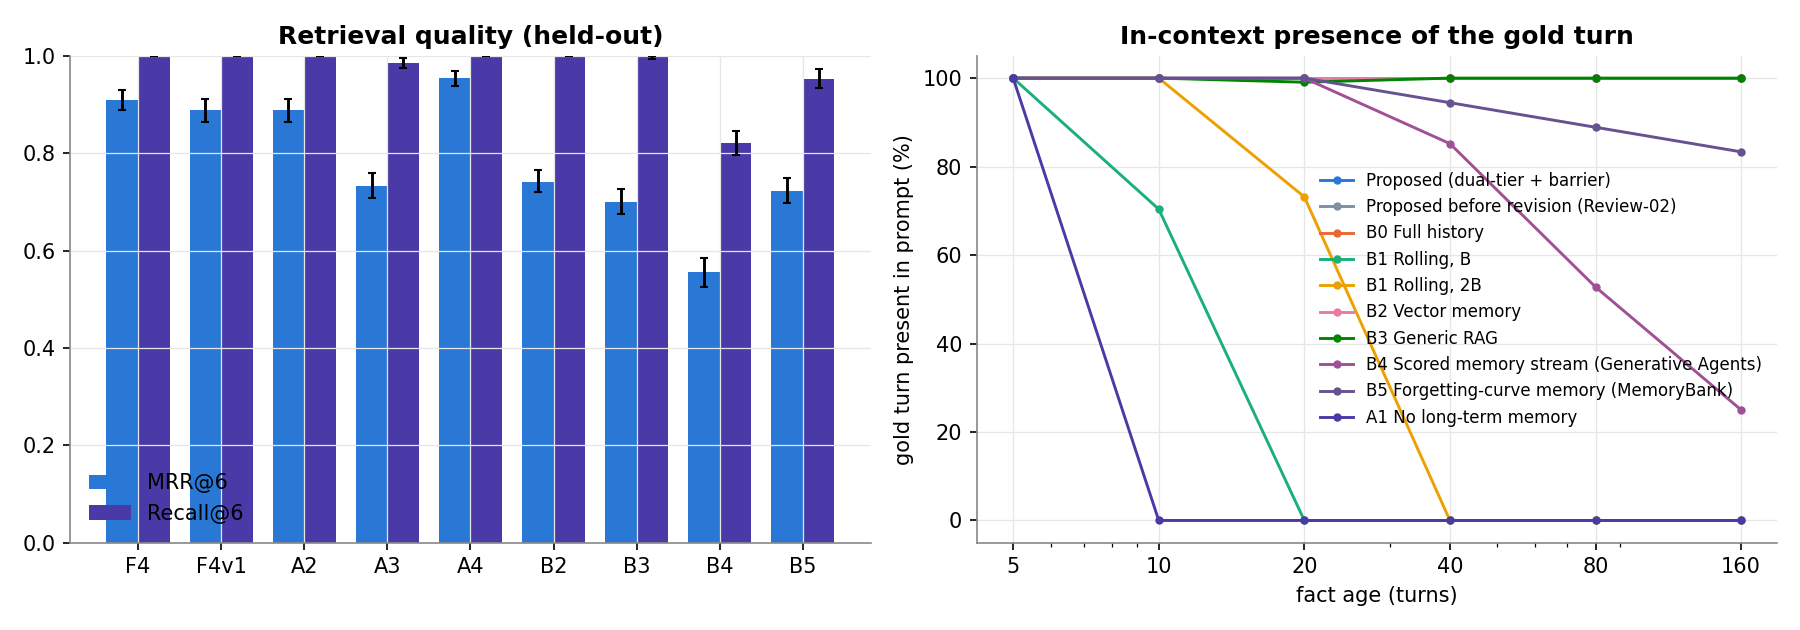
\includegraphics[width=0.82\linewidth]{04_retrieval_quality.png}
\caption{Left: MRR@6 and Recall@6 of the gold memory for each retrieval condition, on the 432 held-out probes older than the buffer. Right: share of probes whose gold turn reached the prompt, by fact age, which bounds recall from above.}
\label{fig:retrieval}
\end{figure}

\Cref{tab:sweeps} lists the sensitivity sweeps plotted in \cref{fig:sweeps}.

\begin{table}[H]
\centering\footnotesize
\caption{Sensitivity sweeps (retrieval only, W1 and W2a to W2c, horizons 100 and 200, 880 probes per setting).}
\label{tab:sweeps}
\begin{tabular}{@{}lccccccc@{}}
\toprule
 & buffer 4 & buffer 8 & buffer 16 & $k=3$ & $k=12$ & $\theta=0$ & $\theta=6$ \\
\midrule
Gold in prompt & 0.9989 & 0.9989 & 0.9989 & 0.9648 & 1.0000 & 1.0000 & 0.9955 \\
MRR@$k$ & 0.8990 & 0.8990 & 0.8990 & 0.8390 & 0.9124 & 0.9227 & 0.8303 \\
\bottomrule
\end{tabular}
\end{table}

\Cref{fig:budget} plots the budget sweep and the trade-off between recall, tokens and latency.

\begin{figure}[H]
\centering
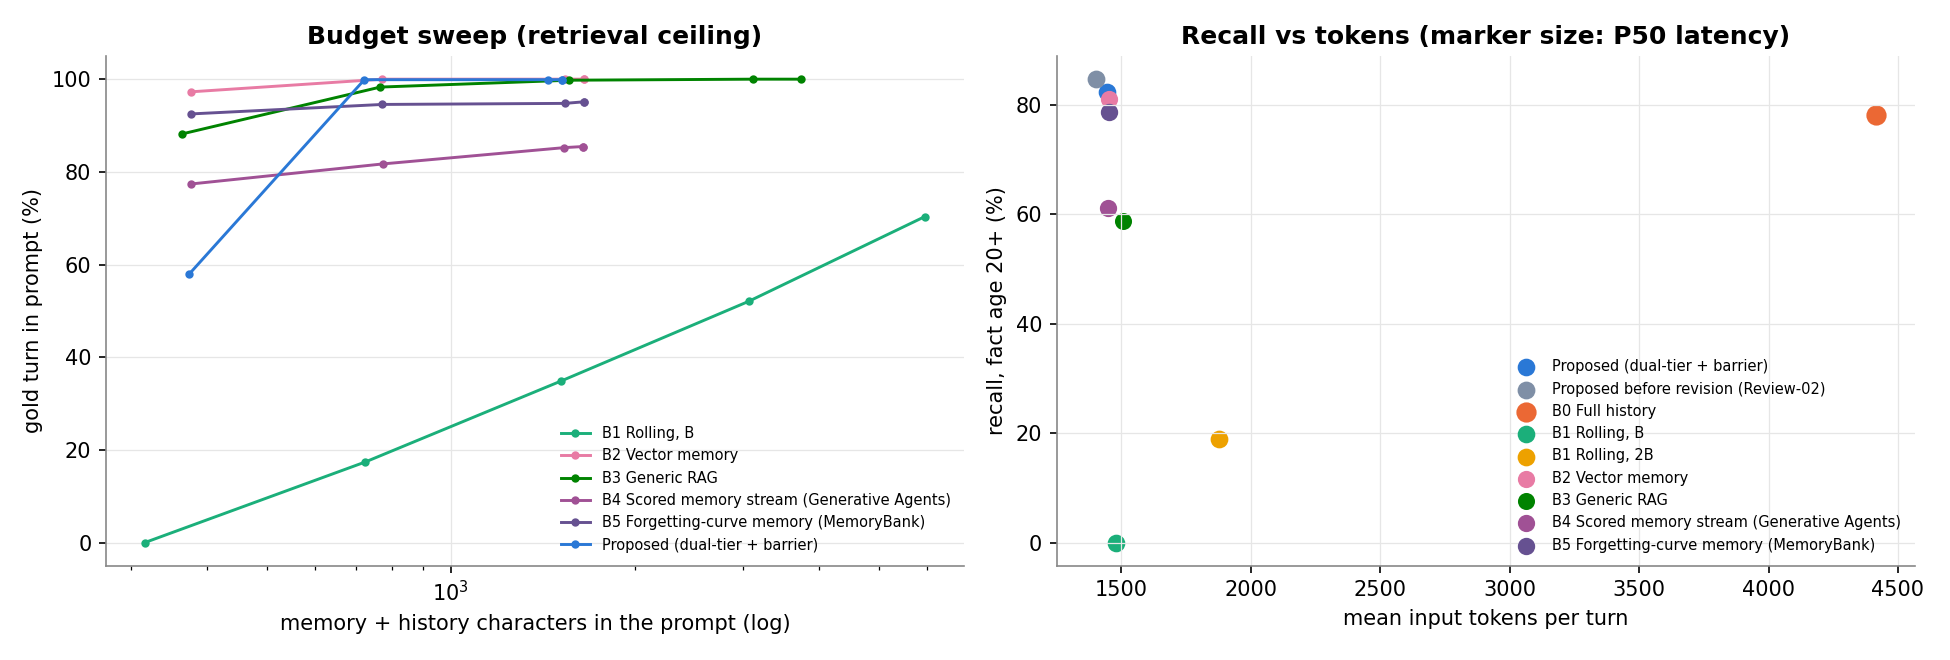
\includegraphics[width=0.82\linewidth]{15_budget_tradeoff.png}
\caption{Left: share of probes whose gold turn reaches the prompt as each condition's budget is scaled from 0.25 to 4 times 1{,}600 characters (CPU sweep on W1 and W2). Right: recall at fact age 20 or more against mean input tokens, with marker size proportional to P50 single-stream latency, which is between 5.9 and 6.9\,s for every condition except B0.}
\label{fig:budget}
\end{figure}

\Cref{fig:codes} breaks the live violations of \cref{tab:factorial} down by invariant.

\begin{figure}[H]
\centering
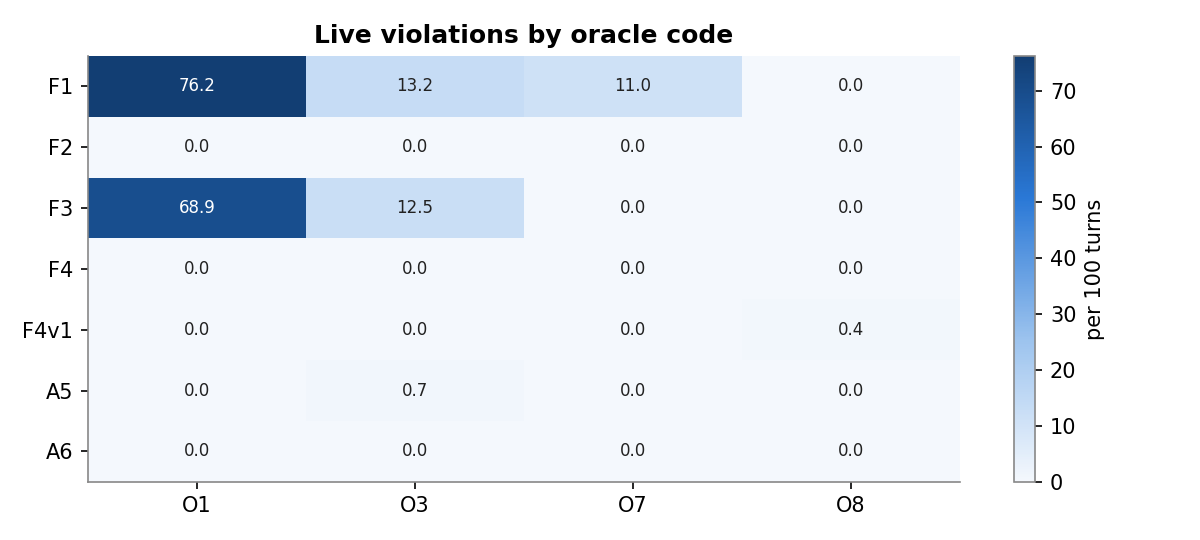
\includegraphics[width=0.82\linewidth]{11_live_violation_codes.png}
\caption{Oracle-flagged live turns per 100 turns by condition and invariant code (codes that never fired are omitted by the plot). Direct writes (F1 and F3) fail on O1, O3 and O7, with a few O5. The corrected-barrier conditions F2 and F4, and A6, have none. A5 has 0.5 O3 and 0.2 O7, and F4v1 0.2 O5 and 0.5 O8 per 100 turns.}
\label{fig:codes}
\end{figure}

\Cref{fig:before-after} plots the main rows of \cref{M-tab:before-after}.

\begin{figure}[H]
\centering
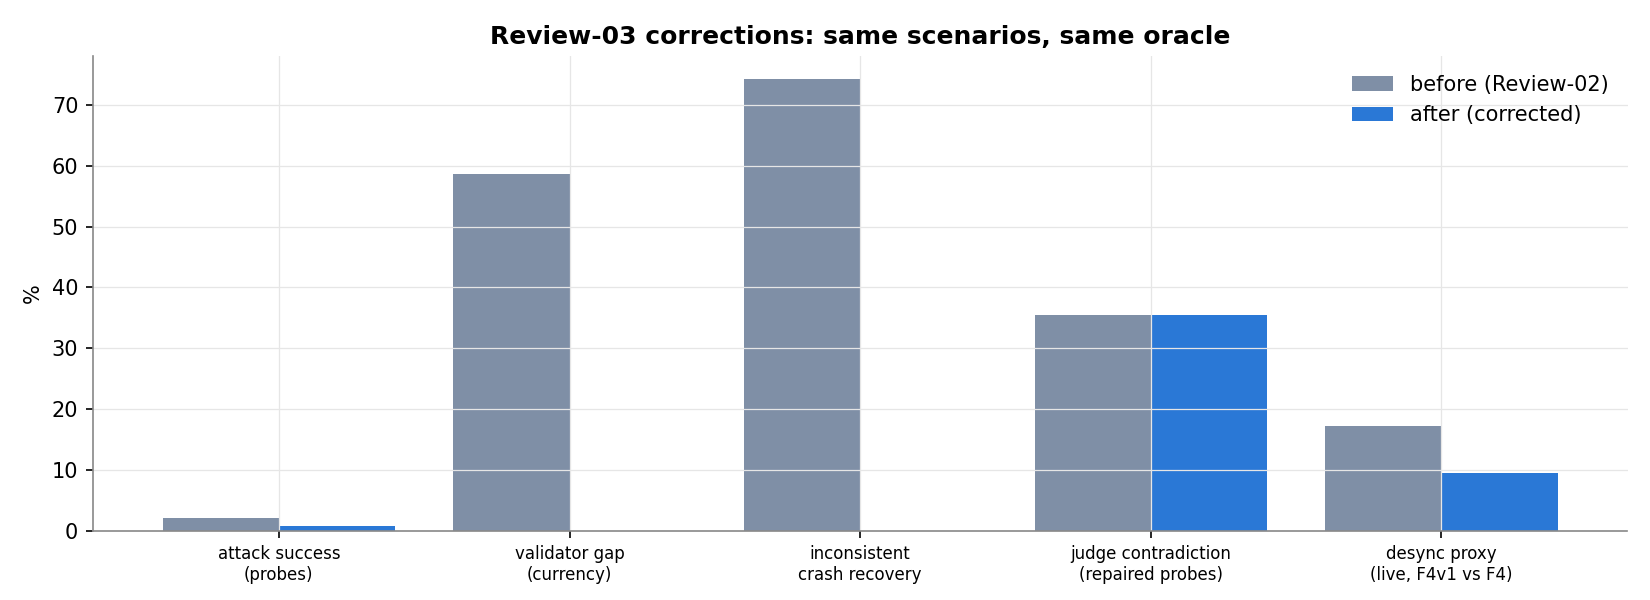
\includegraphics[width=0.82\linewidth]{14_before_after.png}
\caption{Before (Review-02 system, grey) and after (corrected system, blue) on the same scenarios: attack success and currency validator gap under the two validators, inconsistent crash recoveries under the two load paths, judged contradictions of draft and repaired probe replies, and the live desynchronisation proxy of F4v1 and F4.}
\label{fig:before-after}
\end{figure}

\Cref{fig:seeds} plots the seed variance of \cref{tab:seeds} and the recall of all four models on their common subset.

\begin{figure}[H]
\centering
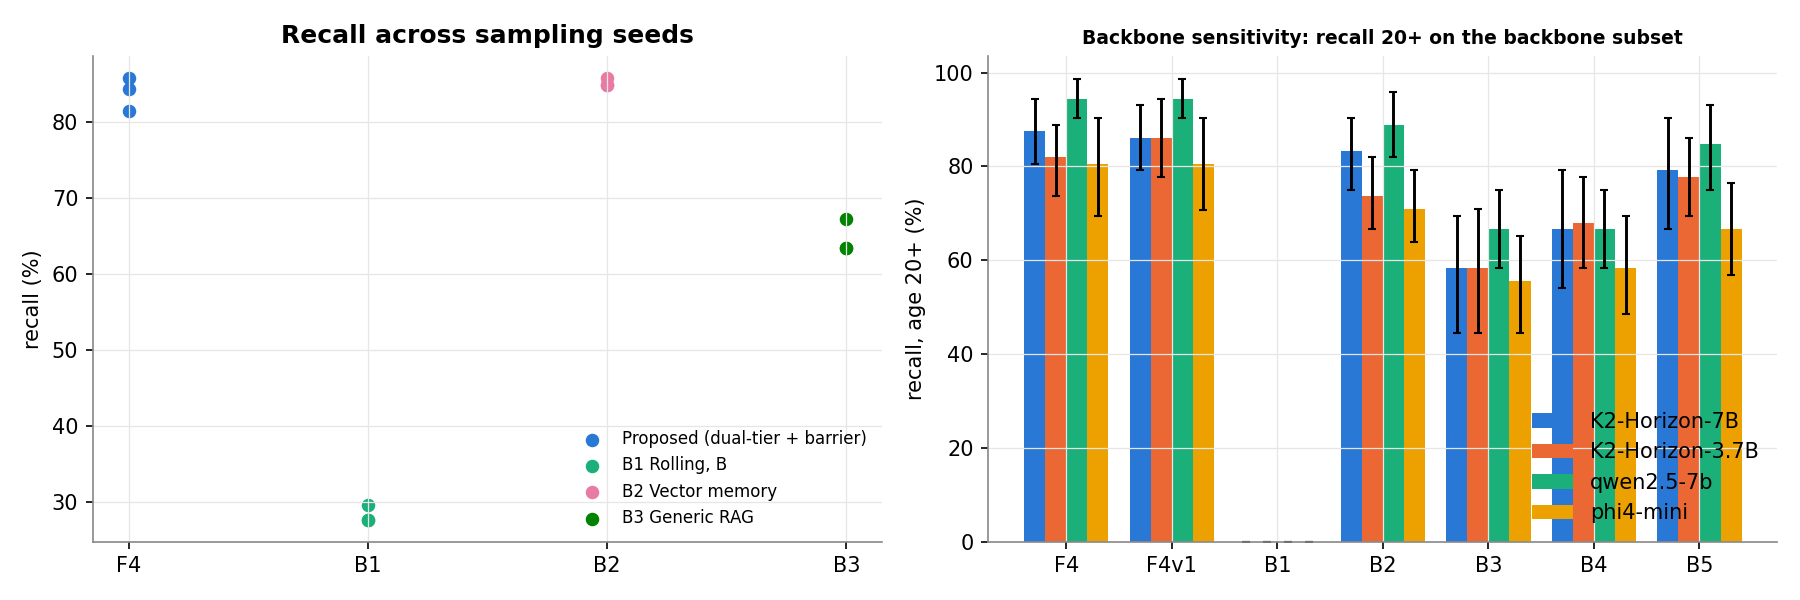
\includegraphics[width=0.82\linewidth]{12_seed_and_backbone.png}
\caption{Left: recall over all ages for three sampling seeds on the calibration sessions. Right: recall at fact age 20 or more on the common subset (W1, W2a, W3, W4-32 at horizon 100, 72 probes per bar) for K2-Horizon-7B, K2-Horizon-3.7B, Qwen2.5-7B and Phi-4-mini. F4 stays between 81\% and 94\% across models and above every baseline for each model.}
\label{fig:seeds}
\end{figure}

\Cref{fig:probes} plots the attack success and validator errors of \cref{M-tab:probes}.

\begin{figure}[H]
\centering
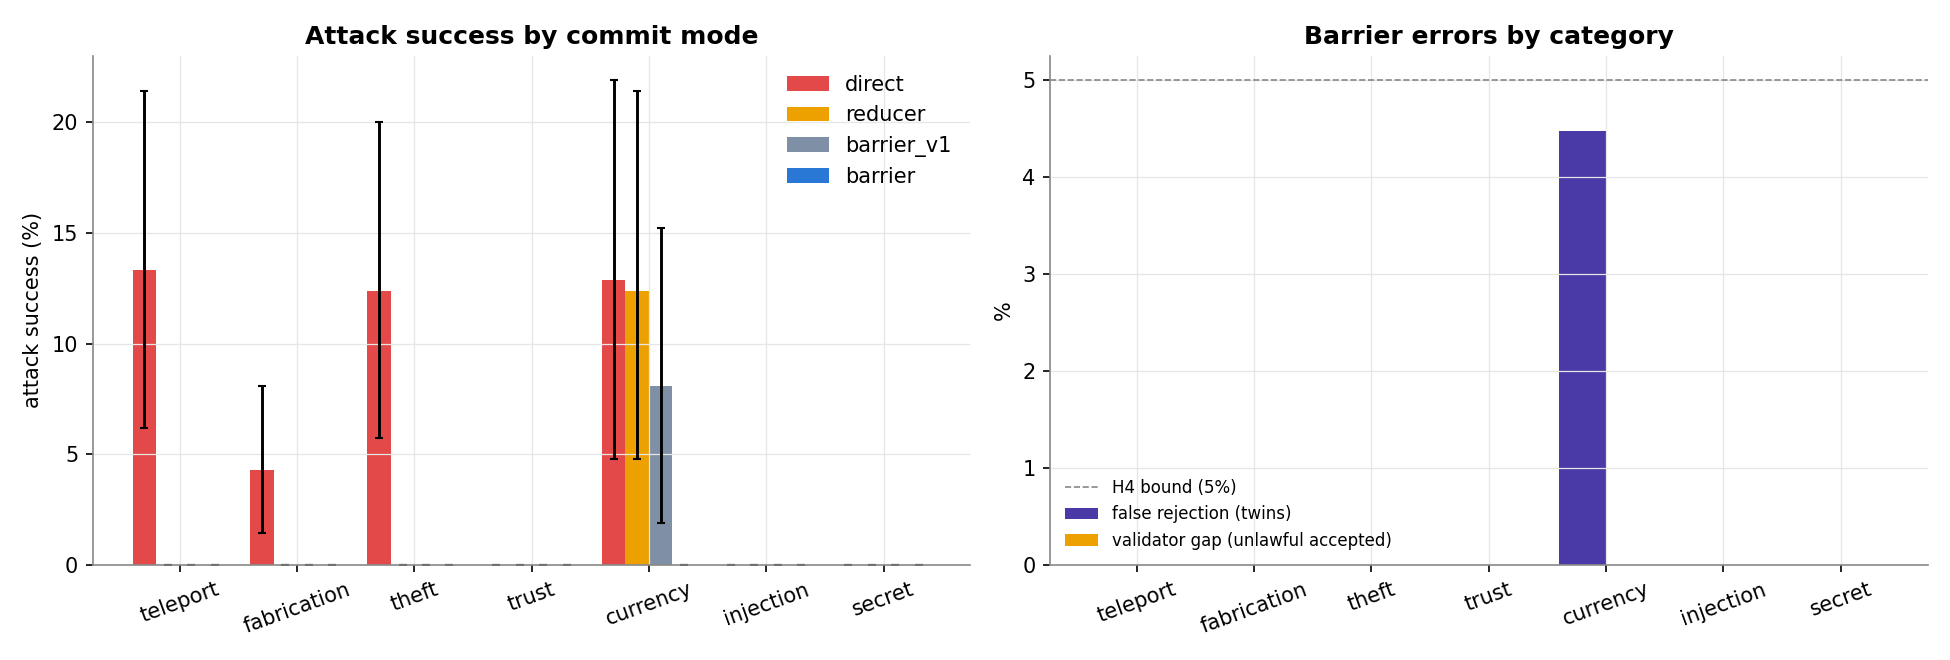
\includegraphics[width=0.82\linewidth]{05_adversarial_probes.png}
\caption{Left: attack success by category when the same model outputs are committed by direct writes, by the reducer without validation (A5), through the Review-02 barrier and through the corrected barrier. Right: the corrected barrier's false rejection of lawful twins (one trust and three currency twin proposals, each naming an NPC by display name, the trust bar is 1 of 14 proposals) and its validator gap (zero in every category), against the 5\% bound of H4.}
\label{fig:probes}
\end{figure}

\Cref{fig:factorial} plots the $2\times2$ cells of \cref{tab:factorial}.

\begin{figure}[H]
\centering
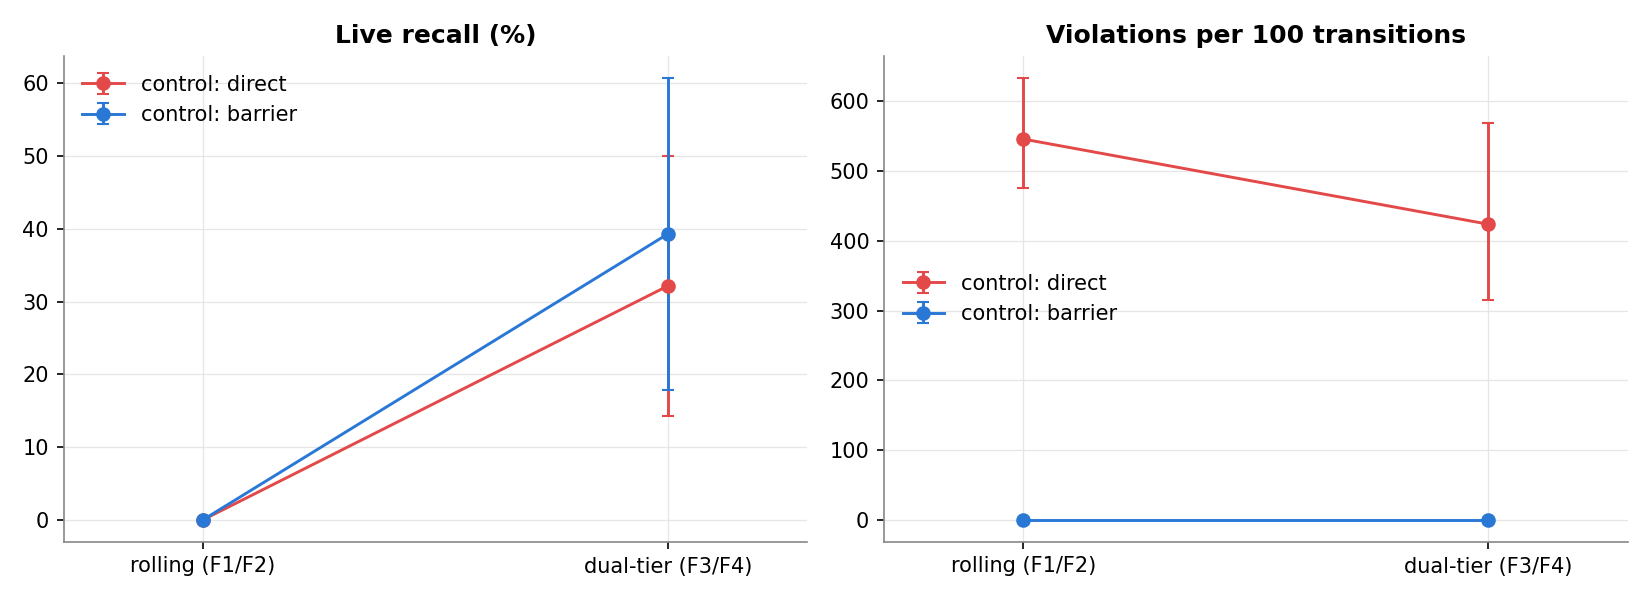
\includegraphics[width=0.82\linewidth]{06_factorial_interaction.png}
\caption{Interaction plots for the $2\times2$ design. Left: live recall rises with memory under either control setting. With dual-tier memory it is 8.9 points higher with the barrier, which the session-level test does not find significant. Right: violations per 100 transitions fall to zero with the barrier under either memory setting. The mixed model (\cref{tab:glmm}) finds a recall interaction.}
\label{fig:factorial}
\end{figure}

\Cref{tab:latency} gives the per-stage latency of the live F4 graph.

\begin{table}[H]
\centering\footnotesize
\caption{Per-stage latency (ms) of the live F4 graph, single stream (24 uncached turns, two worlds). Repair is the dialogue-repair LLM call, needed on 2 of the 24 turns. Local total excludes the LLM and repair calls (\osrc{metrics/table6_stage_latency.csv}).}
\label{tab:latency}
\begin{tabular}{@{}lccccccccccc@{}}
\toprule
 & Input & Retrieval & Prompt & LLM & Parse & Validate & Repair & Commit & Output & Local total & End to end \\
\midrule
P50 & 0.002 & 0.153 & 0.130 & 8{,}113 & 0.087 & 0.013 & 0.002 & 8.427 & 0.010 & 15.101 & 8{,}127 \\
P95 & 0.002 & 0.241 & 0.167 & 14{,}933 & 0.125 & 1.397 & 4{,}491 & 12.980 & 0.012 & 19.210 & 17{,}673 \\
P99 & 0.003 & 0.266 & 0.246 & 15{,}465 & 0.138 & 1.520 & 6{,}516 & 13.388 & 0.013 & 20.393 & 21{,}469 \\
\bottomrule
\end{tabular}
\end{table}

\Cref{fig:latency} plots the stage latencies of \cref{tab:latency} and the single-stream LLM time per condition.

\begin{figure}[H]
\centering
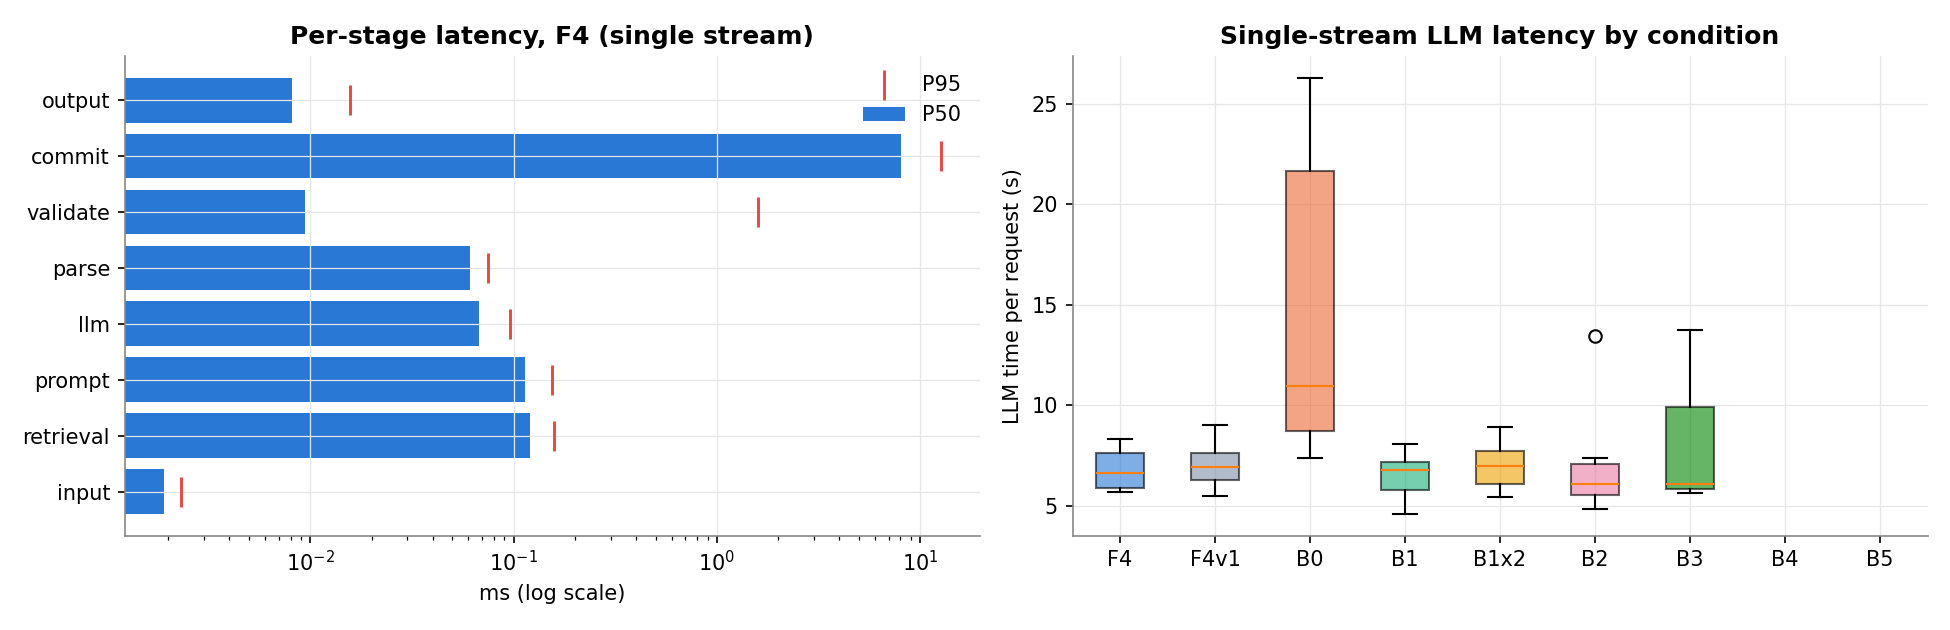
\includegraphics[width=0.82\linewidth]{07_latency.png}
\caption{Left: P50 (bars) and P95 (ticks) latency of each F4 stage, single stream, log scale, including the dialogue-repair stage (\cref{tab:latency}). Right: single-stream LLM time per request for each condition's recall prompts (12 requests per condition).}
\label{fig:latency}
\end{figure}

\Cref{fig:perworld} plots the per-world effects of \cref{tab:perworld}.

\begin{figure}[H]
\centering
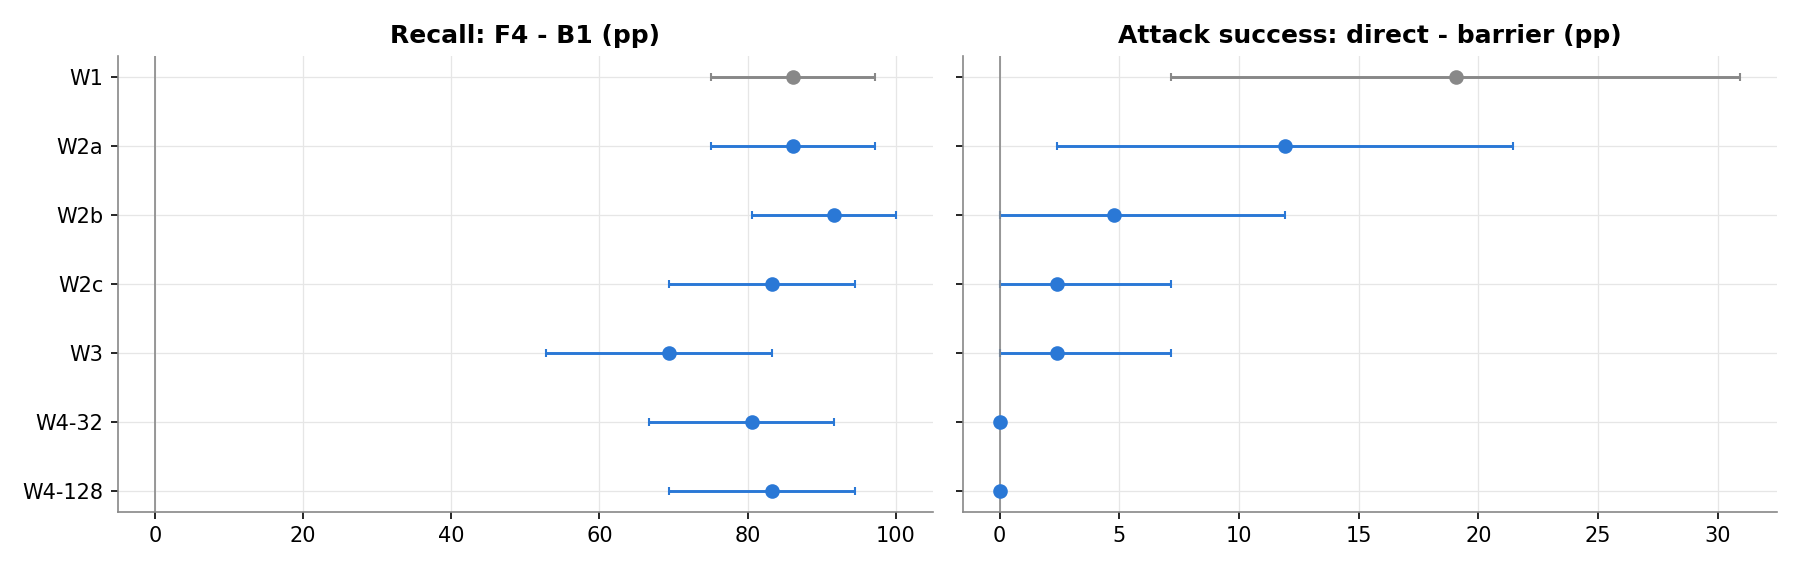
\includegraphics[width=0.82\linewidth]{10_per_world_effects.png}
\caption{Per-world effects with 95\% bootstrap intervals. Left: recall gain of F4 over B1 at fact age 20 or more, positive on every world. Right: reduction in attack success from direct writes to the barrier (F4 context). Positive on W1, W2a to W2c and W3 and zero on W4-32 and W4-128, where no attack succeeded under direct writes. W1 (grey) is in-distribution.}
\label{fig:perworld}
\end{figure}

\Cref{tab:errors} gives the automatically coded failures of \cref{sec:errors}.

\begin{table}[H]
\centering\footnotesize
\setlength{\tabcolsep}{3.5pt}
\caption{Automatically coded failures: recall categories on all worlds (miss: gold not in the prompt, ignored: gold in the prompt, answer wrong, confused: answered with the distractor's value) and live desynchronisation by the proxy. Up to 50 examples per category and condition are exported to \osrc{annotation/error_samples.csv}.}
\label{tab:errors}

\begin{tabular}{@{}lrrrrrrrrrrrr@{}}
\toprule
 & F4 & F4v1 & B0 & B1 & B1$\times$2 & B2 & B3 & B4 & B5 & A1 & A3 & F2 \\
\midrule
Miss & 0 & 0 & 0 & 335 & 220 & 0 & 1 & 65 & 17 & 388 & 6 & -- \\
Ignored & 84 & 53 & 108 & 26 & 51 & 80 & 146 & 68 & 72 & 19 & 109 & -- \\
Confused & 13 & 6 & 32 & 85 & 83 & 2 & 61 & 11 & 5 & 109 & 10 & -- \\
Schema failure & 16 & 5 & 8 & 2 & 6 & 6 & 12 & 17 & 10 & 10 & 6 & -- \\
Desync (live) & 52 & 103 & -- & -- & -- & -- & -- & -- & -- & -- & -- & 68 \\
\bottomrule
\end{tabular}
\end{table}

\section{Sample-Size Ladder}\label{app:ladder}
\Cref{tab:ladder} lists the eight pre-declared sample-size levels of \cref{sec:repro}.

\begin{table}[H]
\centering\footnotesize
\caption{Pre-declared sample-size levels and the planner's estimated hours for the reported run (\osrc{metrics/budget_plan.csv}). Level 2 was run. Its four LLM stages took 5.49\,h against 6.76\,h estimated.}
\label{tab:ladder}
\begin{adjustbox}{max width=\linewidth}
\begin{tabular}{@{}crrrrrrrr@{}}
\toprule
Level & Sessions/(world, $H$) & Probes/(world, cat.) & Live/world & Recall (h) & Probes (h) & Live (h) & Seed var.\ (h) & Total (h) \\
\midrule
0 & 1 & 4 & 1 & 0.90 & 0.60 & 0.89 & 0.54 & 2.94 \\
1 & 2 & 6 & 1 & 1.86 & 0.94 & 0.89 & 0.54 & 4.24 \\
\textbf{2} & \textbf{3} & \textbf{10} & \textbf{2} & \textbf{2.82} & \textbf{1.62} & \textbf{1.77} & \textbf{0.54} & \textbf{6.76} \\
3 & 4 & 14 & 2 & 3.78 & 2.30 & 1.77 & 0.54 & 8.40 \\
4 & 6 & 20 & 3 & 5.71 & 3.32 & 2.66 & 0.54 & 12.23 \\
5 & 10 & 30 & 4 & 9.55 & 5.01 & 3.54 & 0.54 & 18.65 \\
6 & 20 & 45 & 6 & 19.15 & 7.55 & 4.43 & 0.54 & 31.68 \\
7 & 40 & 60 & 10 & 38.37 & 10.10 & 7.09 & 0.54 & 56.10 \\
\bottomrule
\end{tabular}
\end{adjustbox}
\end{table}

% The supplement's own reference list numbers its citations independently of the manuscript's.
\bibliographystyle{IEEEtran}
\bibliography{references}

\end{document}
